%ARCHIVO PRINCIPAL DE LATEX
%10 DE SEPTIEMBRE DEL 2021
%SOFTWARE MANTENIMIENTO DE AUTOS

\documentclass[letterpaper,11pt]{report} 
\usepackage[utf8]{inputenc} %Caracteres: UTF8
\usepackage[spanish]{babel} %Lenguaje: Espanol
\usepackage{graphicx}%Manejo de imagenes
\usepackage{appendix}%Manejo de apendices (anexos)

\begin{document}
	\renewcommand{\tablename}{Tabla}
	\renewcommand{\listtablename}{Índice de tablas}
	\begin{titlepage}
	
	\centering %Todo centrado
	
	%%%%  LOGO DE LA ESCUELA   %%%%
	
\includegraphics[scale=0.2]{imagenes/ipn} %Imagen para portada
	
\includegraphics[scale=0.65]{imagenes/upiicsa} %Imagen para portada
	%%%%  NOMBRE DE LA ESCUELA   %%%%
	\LARGE \textbf{\\ Instituto Politécnico Nacional}
	\LARGE \textbf{\\ Unidad Profesional Interdisciplinaria de Ingeniería y Ciencias Sociales y Administrativas}
	
	\vspace{1cm} %Espacio vertical
	
	\large \textbf{SOFTWARE PARA APOYAR A LA LOGÍSTICA DEL MANTENIMIENTO DE AUTOMÓVILES}% Materia
	
	\vspace{1cm} %Espacio vertical
	
	%%%%%%  TRABAJO REALIZADO   %%%%%%
	\large \textbf{CALIDAD Y NORMALIZACIÓN DE SOFTWARE}\\% Unidad
	\rule{13cm}{3pt} % Linea horizontal
	\large \textbf{\\ INGENIERÍA EN INFORMÁTICA} %Trabajo
	
	\vspace{1cm} %Espacio vertical
	
	%%%%   ALUMNOS   %%%%
	\textbf{Elaborado por:}\\
	\vspace{0.5cm} %Espacio vertical
	\textit \textbf{EQUIPO 7}\\
	Guzmán Montero Aura Regina \hspace{2cm} 2012600652\\
	Ibarra Ferrer Eliot Ramón \hspace {3cm} 2015070649\\ 
	Reyna Cruz Emmanuel \hspace{3.5cm} 2018602051\\
	Núñez Hernández Ulises \hspace{3.5cm} 2014121002\\

	\vspace{1cm} %Espacio vertical
	
	4NM81
	
	\vspace{1cm} %Espacio vertical
	
	\today
	
\end{titlepage} %Se inserta portada
	\begin{abstract}
	El presente documento contiene la especificación tanto del análisis como el diseño de un sistema de información que permite la gestión de refacciones automotrices así como la agenda de los trabajos y/o procesos que se realizan en un taller mecánico y mantenimiento vehicular dentro de la empresa 'Productos Plazco S.A.'. 
	\\En cuanto al análisis, se presentan historias de usuario que nos describen como es que las tareas que se realizan actualmente, se modificarán con ayuda del software. En la parte de diseño, mostramos toda la parte de la arquitectura se implementa el modelo de vistas 4+1: vista de procesos, vista física, vista de desarrollo, vista lógica y vista de escenarios. En esta última se describe a detalle el comportamiento de cada escenario planteado en la aplicación. 
\end{abstract} %Se inserta resumen
	\pagestyle{headings}
	
	\tableofcontents %Tabla de contenidos
	\listoffigures %Tabla de imagenes
	\listoftables%Lista de tablas
	\clearpage %Acomodar por página
	
	%Contenido
	\chapter{Introducción}
A continuación se explica de manera detallada cada uno de los elementos de la introducción del presente documento.

%Contenido del capítulo de introducción
\section{Problemática}
En la empresa Productos Plazco S.A, presentan diversos problemas dentro del área de mantenimiento vehicular. Se registra que dentro del periodo Enero-Diciembre de 2019 se encontraron fallas en los siguientes procesos:
\begin{itemize}
	\item Mal control de inventario para las refacciones que se llegan a utilizar para el mantenimiento de los vehículos .
	\item No se lleva un registro de las entradas y salidas de los vehículos.
	\item Falta de especificación del trabajo al momento de ingresar un vehículo.
	\item Desfase en los tiempos de trabajo. No se cuenta con un protocolo para la definición de los trabajos a realizar por lo que algunas actividades tardan mas de lo deseado.
	\item Mala asignación para la realización de tareas.
	\item Mala comunicación con los conductores de cada unidad
	Todas estas fallas se deben a que no se lleva un buen control, ni una buena administración para la asignación de tareas, al igual que se detecta una falta de organización al momento de el registro de inventarios y una falla en la comunicación con los choferes de cada unidad vehicular. De la misma forma el principal problema que se detecta es al momento de ingresar las unidades al taller ya que no se define desde un inicio el trabajo que se debe realizar, el tiempo estimado y las personas responsables del mismo, esto genera un tiempo excesivo para el mantenimiento de cada vehículo y una pérdida del control en las refacciones necesarias para cada trabajo.
\end{itemize}
\section{Solución}
La solución que se propone es la implementación de un sistema desarrollado en Java, la ventaja de realizarlo así es la JVM la cual nos permitirá ejecutar la aplicación en cualquier sistema operativo, al igual de poder implementar una aplicación más robusta. 
\\
Nuestro sistema ofrece las siguientes características:
\begin{itemize}
	\item Inicio de sesión para permitir el acceso solo a los usuarios que cuenten con credenciales válidas. 
	\item Un menú que permita la fácil navegación dentro del sistema.
	\item Un apartado de registro para poder controlar la entrada de cada vehículo.
	\subitem Se permitirá modificar la información de un vehículo que se encuentre previamente registrado dentro del sistema.
	\subitem Se podrá eliminar el registro de un vehículo.
	\subitem Se podrá buscar el registro individual de cada vehículo.
	\item Permitirá visualizar las refacciones con las que se cuenta.
	\item Permitirá la solicitud de las refacciones disponibles, de esta forma se podrá llevar un control de estas.
	\item El manejo de una base de datos para el almacenamiento de toda la información que se registre.
\end{itemize}
\clearpage
\section{Objetivo}
Desarrollar un sistema que permita el control de inventarios de refacciones, incluyendo un apartado para realizar las solicitudes para un mejor manejo de las refacciones disponibles y registro de los servicios que se realizan a cada automóvil, así como el control de las personas encargadas de cada servicio, fechas de entrada y fechas de salida de las unidades. 
\section{Alcance}
Lo que se busca en la realización de este proyecto es optimizar los procesos que se brindan en el área de mantenimiento vehicular, así como mejorar el control que se lleva en los inventarios, dando así   una mejor optimización de las refacciones disponibles y una aceleración en las tareas que se deben realizar.
\\
En el primer entregable de este proyecto se busca realizar la entrega de un MVP (Producto Mínimo Viable), de esta forma buscamos entregar en un lapso corto de tiempo y ver la aceptación que se tiene de este, así como recopilar información para próximas iteraciones en donde se buscará un avance gradual del sistema hasta que se cuente con un producto terminado al 100%

	\chapter{Análisis de Datos}
En este capítulo se desglosan de manera detallada los requerimientos funcionales y no funcionales del software que se va a desarrollar.

\section{Requerimientos Funcionales}
Al analizar la problemática que presenta el cliente, llegamos a un listado de los siguientes requerimientos funcionales del proyecto: 
\begin{itemize}
	\item El sistema permitirá el acceso si y solo si se ingresan de manera correcta las credenciales solicitadas, además de que exista el usuario en la base de datos.
	\item El sistema desplegará un menú donde el usuario podrá elegir si gestiona la agenda de vehículos o las refacciones. 
	\item El sistema mostrará en una pantalla todos aquellos registros de vehículos que el usuario tenga relacionados. 
	\item El sistema permitirá al usuario registrar, modificar, eliminar y buscar un registro por medio de formularios. 
	\item El sistema validará todas y cada una de las entradas de datos, en caso de que estas sean erróneas, se mostrará un mensaje de alerta. 
	\item El sistema mostrará en pantalla todos aquellos registros de refacciones que haya en existencia dentro del almacén del taller. 
	\item El sistema permitirá al usuario solicitar una refacción por medio de un formulario de registro. 
\end{itemize}
\section{Requerimientos No Funcionales}
Estos requerimientos no intervienen en la funcionalidad del sistema, sin embargo, es importante tomarlos en cuenta ya que se expresan algunas características fundamentales del propio sistema.
\begin{itemize}
	\item La interfaz gráfica de usuario (GUI) debe de estar bien diseñada en cada una de la pantallas.
	\item Será desarrollado en el lenguaje de programación Java con ayuda del IDE Apache Netbeans en su versión 12.4. Esto para aprovechar que el lenguaje soporta multiplataforma además de que la curva de aprendizaje ya esta dada. 
	\item La base de datos será desarrollada en MySQL y será montada en el servidor un servidor local con ayuda de XAMPP en su versión 3.2.4 para las pruebas del MVP. 
\end{itemize}
	\chapter{Análisis} \label{chap: historias de usuario}
En este capítulo se desarrollaron Historias de Usuario donde se describen a detalle la interacción y/o las acciones que cada uno de los actores se verá envuelto. Para poder identificar dichas historias, se empleará la nomenclatura HU'X' donde 'X' es el número de historia de usuario que se esta describiendo.
\\
Cada historia de usuario contiene la siguiente información:

\begin{itemize}
	\item Usuario: Nombre del usuario
	\item Responsable: Nombre de la persona con quien se revisó la historia de usuario
	\item Elaborada por: Nombre de quien elaboró la historia de usuario
	\item Descripción:
\end{itemize}

	\textbf{Como} \textless USUARIO\textgreater \textbf{debo de poder}\textless ACCION\textgreater \textbf{para que}\textless BENEFICIO\textgreater

\clearpage
%Contenido de las historias de usuario
\section{Entregables}

En la tabla \ref{tab: Listado de Historias de Usuario Entregadas} se listan las Historias de Usuario entregadas en el presente documento.

\begin{table}[h]
	\begin{center}
		\begin{tabular}{|c|c|c|c|c|}
			\hline 
			\textbf{Id} & \textbf{Nombre} & \textbf{Reunión} \\ 
			\hline 
			HU1  & Iniciar Sesión  & --------  \\
			HU2  & Visualizar Menú  & --------  \\ 
			HU3  & Visualizar Agenda  & --------  \\
			HU4  & Registrar Entrada de Vehículo  & --------  \\
			HU5  & Modificar Registro de Vehículo  & --------  \\
			HU6  & Eliminar Registro de Vehículo  & --------  \\
			HU7  & Buscar Registro de Vehículo  & --------  \\
			HU8  & Visualizar Refacciones Disponibles  & --------  \\
			HU9  & Solicitar Refacción  & --------  \\
			\hline 
		\end{tabular}
	\end{center}
	\label{tab: Listado de Historias de Usuario Entregadas}
	\caption{Listado de Historias de Usuario Entregadas}
\end{table}

La descripción de cada una de las historias de usuario se muestra a continuación.
\clearpage
\section{HU1 Iniciar Sesión}
	\begin{itemize}
	\item Usuario: Mecánico
	\item Responsable: Guzmán Montero Aura Regina
	\item Elaborado por: Núñez Hernández Ulises
	\item Descripción:\\
\end{itemize}

\textbf{Como} mecánico \textbf{debo de poder} iniciar sesión en el sistema con el nombre de usuario y la contraseña que me proporcione la administración de la empresa \textbf{para que} pueda realizar la gestión de los trabajos que entren al taller así como la gestión de las diversas refacciones que necesitaré. 
\vspace{3cm}
\section{HU2 Visualizar Menú}
\begin{itemize}
	\item Usuario: Mecánico
	\item Responsable: Guzmán Montero Aura Regina
	\item Elaborado por: Núñez Hernández Ulises
	\item Descripción:\\
\end{itemize}

\textbf{Como} mecánico \textbf{debo de poder} visualizar un menú una vez que inicie mi sesión en el sistema, en este menú podré elegir entre gestionar la agenda (entradas y salidas de vehículos al taller) \textbf{para que} se desplieguen las pantallas de acuerdo a la opción que elija y poder realizar las actividades que debo llevar a cabo dentro del sistema.
\clearpage
\section{HU3 Visualizar Agenda}
\begin{itemize}
	\item Usuario: Empleado
	\item Responsable: Guzmán Montero Aura Regina
	\item Elaborado por: Núñez Hernández Ulises
	\item Descripción:\\
\end{itemize}

\textbf{Como} Empleado \textbf{debo de poder} visualizar la agenda de todos los trabajos que hay que realizar dentro del taller, estos registros deben de contener todos los datos \textbf{para que} pueda identificar correctamente los vehículos y trabajar en ellos, además de gestionar cada uno de los registros.
\vspace{3cm}
\section{HU4 Registrar Entrada de Vehículo}
\begin{itemize}
	\item Usuario: Mecánico
	\item Responsable: Guzmán Montero Aura Regina
	\item Elaborado por: Núñez Hernández Ulises
	\item Descripción:\\
\end{itemize}

\textbf{Como} mecánico \textbf{debo de poder} registrar la entrada de un vehículo al taller, recabando los datos necesarios del conductor, del vehículo y la problemática a resolver \textbf{para que} se pueda llevar una buena gestión dentro del sistema además de estimar un tiempo de entrada y salida del vehículo en el taller. 
\clearpage
\section{HU5 Modificar Registro de Vehículo}
\begin{itemize}
	\item Usuario: Empleado, Administrador
	\item Responsable: Guzmán Montero Aura Regina
	\item Elaborado por: Núñez Hernández Ulises
	\item Descripción:\\
\end{itemize}

\textbf{Como} empleado o administrador \textbf{debo de poder} modificar cada uno de los registros de los vehículos que han entrado al taller, \textbf{para que} se pueda corregir algún desperfecto al momento de capturar datos o por alguna cuestión externa al taller se deba de modificar la fecha de salida al vehículo.
\vspace{3cm}
\section{HU6 Eliminar Registro de Vehículo}
\begin{itemize}
	\item Usuario: Mecánico
	\item Responsable: Guzmán Montero Aura Regina
	\item Elaborado por: Núñez Hernández Ulises
	\item Descripción:\\
\end{itemize}

\textbf{Como} mecánico \textbf{debo de poder} eliminar uno o varios registros de los vehículos que se han registrado en el sistema \textbf{para que} al momento de terminar el trabajo en algún vehículo, se pueda eliminar este registro y dar entrada a otro más para tener un mejor control. 
\clearpage
\section{HU7 Buscar Registro de Vehículo}
\begin{itemize}
	\item Usuario: Empleado o Administrador
	\item Responsable: Guzmán Montero Aura Regina
	\item Elaborado por: Núñez Hernández Ulises
	\item Descripción:\\
\end{itemize}

\textbf{Como} empleado o administrador \textbf{debo de poder} buscar un registro de algún vehículo por medio de algún dato relevante \textbf{para que} se pueda ahorrar tiempo en la búsqueda de algún vehículo en específico y se realicen las acciones necesarias dentro del sistema. 
\vspace{3cm}
\section{HU8 Visualizar Refacciones Disponibles}
\begin{itemize}
	\item Usuario: Empleado o Administrador
	\item Responsable: Guzmán Montero Aura Regina
	\item Elaborado por: Núñez Hernández Ulises
	\item Descripción:\\
\end{itemize}

\textbf{Como} empleado o administrador \textbf{debo de poder} visualizar las refacciones que hay disponibles dentro del almacén de las instalaciones del taller y usarla en algún trabajo para un vehículo \textbf{para que} se lleve una correcta gestión de las mismas y en caso de que no haya en existencia en almacén, se pueda solicitar una (en el caso del empleado). 
\clearpage
\section{HU2 Solicitar Refacciones}
\begin{itemize}
	\item Usuario: Mecánico
	\item Responsable: Guzmán Montero Aura Regina
	\item Elaborado por: Núñez Hernández Ulises
	\item Descripción:\\
\end{itemize}

\textbf{Como} mecánico \textbf{debo de poder} solicitar alguna refacción que necesite y no esté en el registro del almacén \textbf{para que} la administración obtenga dicha refacción y pueda utilizarla en el vehículo que la necesite. 
\vspace{3cm}
\section{HU10 Visualizar Empleados}
\begin{itemize}
	\item Usuario: Administrador
	\item Responsable: Guzmán Montero Aura Regina
	\item Elaborado por: Núñez Hernández Ulises
	\item Descripción:\\
\end{itemize}

\textbf{Como} administrador \textbf{debo de poder} visualizar una lista de todos los empleados (mecánicos) que hay registrados dentro de la base de datos\textbf{para que} se pueda tener un mejor control sobre sus datos y su trabajo en el taller.
\clearpage
\section{HU11 Registrar Empleados}
\begin{itemize}
	\item Usuario: Administrador
	\item Responsable: Guzmán Montero Aura Regina
	\item Elaborado por: Núñez Hernández Ulises
	\item Descripción:\\
\end{itemize}

\textbf{Como} administrador \textbf{debo de poder} registrar a nuevos empleados (mecánicos) que lleguen al taller \textbf{para que} se pueda tener un mejor control sobre sus datos y su trabajo en el taller.
\vspace{3cm}
\section{HU12 Modificar Empleados}
\begin{itemize}
	\item Usuario: Administrador
	\item Responsable: Guzmán Montero Aura Regina
	\item Elaborado por: Núñez Hernández Ulises
	\item Descripción:\\
\end{itemize}

\textbf{Como} administrador \textbf{debo de poder} modificar algún registro de todos los empleados que están dentro de la base de datos \textbf{para que} en caso de que exista un error en sus datos o en uno de sus trabajos, se pueda corregir de inmediato.
\clearpage
\section{HU13 Eliminar Empleados}
\begin{itemize}
	\item Usuario: Administrador
	\item Responsable: Guzmán Montero Aura Regina
	\item Elaborado por: Núñez Hernández Ulises
	\item Descripción:\\
\end{itemize}

\textbf{Como} administrador \textbf{debo de poder} eliminar algún registro de un empleado que ya no pertenezca al personal del taller \textbf{para que} no exista alguna confusión dentro de la organización y sobre todo tener integridad y limpieza en la base de datos.
\vspace{3cm}
\section{HU13 Buscar Empleado}
\begin{itemize}
	\item Usuario: Administrador
	\item Responsable: Guzmán Montero Aura Regina
	\item Elaborado por: Núñez Hernández Ulises
	\item Descripción:\\
\end{itemize}

\textbf{Como} administrador \textbf{debo de poder} buscar el registro de un empleado dentro del sistema \textbf{para que} se pueda realizar alguna tarea en específico sobre los datos de ese empleado de manera fácil y eficiente.
\clearpage
\section{HU14 Visualizar Solicitud}
\begin{itemize}
	\item Usuario: Administrador
	\item Responsable: Guzmán Montero Aura Regina
	\item Elaborado por: Núñez Hernández Ulises
	\item Descripción:\\
\end{itemize}

\textbf{Como} administrador \textbf{debo de poder} visualizar todas las solicitudes de refacciones de cada uno de los empleados \textbf{para que} se puedan atender a cada una y sea más eficiente la entrega y la disponibilidad de las mismas.
\vspace{3cm}
\section{HU16 Atender Solicitud}
\begin{itemize}
	\item Usuario: Administrador
	\item Responsable: Guzmán Montero Aura Regina
	\item Elaborado por: Núñez Hernández Ulises
	\item Descripción:\\
\end{itemize}

\textbf{Como} administrador \textbf{debo de poder} atender cada una de las solicitudes de refacciones que los empleados han llenado  \textbf{para que} se consiga con proveedores la refacción necesaria y se coloque dentro del almacén y el empleado pueda utilizarla.  
\clearpage
\section{HU17 Registrar Refacciones}
\begin{itemize}
	\item Usuario: Administrador
	\item Responsable: Guzmán Montero Aura Regina
	\item Elaborado por: Núñez Hernández Ulises
	\item Descripción:\\
\end{itemize}

\textbf{Como} administrador \textbf{debo de poder} registrar nuevas refacciones que lleguen al almacén aun que estas no hayan sido solicitadas \textbf{para que} la disponibilidad de cada reacción sea mayor y los empleados puedan realizar su trabajo en tiempo y forma.
\vspace{3cm}
\section{HU18 Modificar Refacciones}
\begin{itemize}
	\item Usuario: Administrador
	\item Responsable: Guzmán Montero Aura Regina
	\item Elaborado por: Núñez Hernández Ulises
	\item Descripción:\\
\end{itemize}

\textbf{Como} administrador \textbf{debo de poder} modificar el registro de alguna reacción que esté dentro del alamcén \textbf{para que} en dado caso que exista un error en la captura, se pueda modificar la información de inmediato. 
\clearpage
\section{HU19 Eliminar Refacciones}
\begin{itemize}
	\item Usuario: Administrador
	\item Responsable: Guzmán Montero Aura Regina
	\item Elaborado por: Núñez Hernández Ulises
	\item Descripción:\\
\end{itemize}

\textbf{Como} administrador \textbf{debo de poder} eliminar un registro de alguna refacción que esté dentro del almacén en dado caso que el proveedor no la tenga o no haya en existencia \textbf{para que} no haya una confusión con los empleados.
\vspace{3cm}
\section{HU20 Buscar Registro de Refacciones}
\begin{itemize}
	\item Usuario: Empleado, Administrador
	\item Responsable: Guzmán Montero Aura Regina
	\item Elaborado por: Núñez Hernández Ulises
	\item Descripción:\\
\end{itemize}

\textbf{Como} empleado o administrador \textbf{debo de poder} buscar algún registro de una refacción que se encuentre dentro de almacén \textbf{para que} la búsqueda sea más rápida y eficiente.
	\chapter{Diseño}
En este capítulo se describe la arquitectura a utilizar y los diversos diagramas que implican el diseño del sistema a implementar para darle solución a la problemática.

%Contenido del capítulo Diseño
\section{Arquitectura del Software}
El modelo de arquitectura 4+1 fue diseñado por Philippe Kruchten para poder describir la arquitectura de sistemas de software, basados en el uso de múltiples vistas, dichas vistas describen el sistema desde diferentes puntos de vista como de usuario final o desarrolladores. \\
Las cuatro vistas de este modelo son:
\begin{itemize}
	\item \textbf{Vista de Procesos:} Trata los aspectos dinámicos del sistema y como su nombre lo dice, explica todos los procesos del sistema y como es que se comunica el actor con el sistema.
	\item \textbf{Vista Lógica:} Enfocada a describir la estructura y funcionalidad de un sistema con ayuda de diagramas UML como Diagramas de Clase o de Secuencia.

	\item \textbf{Vista de Desarrollo:} Muestra el sistema desde el punto de vista de un programador. Se plasman las interfaces que se van a utilizar y el enlace entre cada una. Se utilizan Diagramas de Componentes o de Paquetes.
	\item \textbf{Vista Física:} Esta relacionado con la topología de componentes de hardware que se implementan para poder utilizar el sistema o aplicación. Muestra los componentes físicos como computadoras, redes, nodos, etc.
	\item \textbf{Vista de Escenarios:} Utilizando Casos de Uso, describe secuencias de interacciones entre objetos y procesos.
\end{itemize}

En la figura \ref{fig:Modelo de Arquitectura 4+1: Kruchten} nos muestra como es que se ha diseñado este modelo:
\begin{figure}[!h]
	\centering
	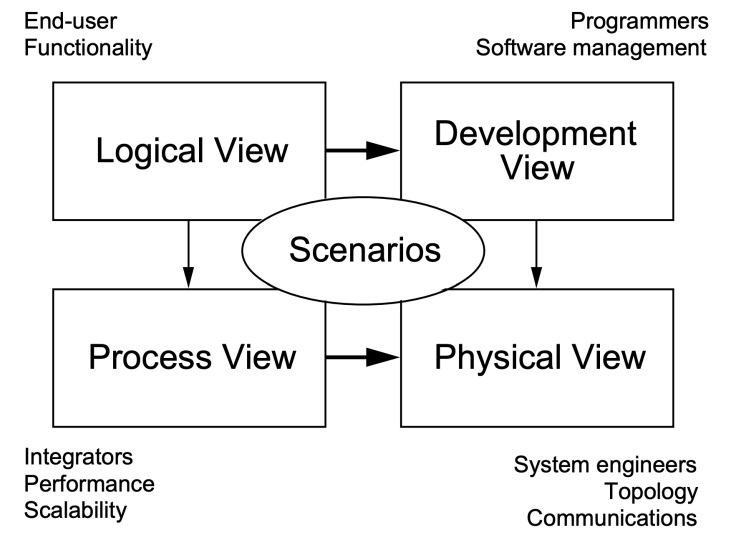
\includegraphics[width=1\textwidth]{./diseno/arquitectura/imagenes/arquitectura}
	\caption{Modelo de Arquitectura 4+1: Kruchten}
	\label{fig:Modelo de Arquitectura 4+1: Kruchten}
\end{figure}

\clearpage
\section{Vista de Procesos}
A continuación se muestran los diagramas de secuencia diseñados para la interacción entre el usuario ('administrador' y 'empleado') y el sistema de información. 

%Contenido de la vista de procesos
\subsection{Vista de Procesos Empleado} \label{subsec: Vista Procesos Empleado}
\subsubsection{Iniciar Sesión}
En la figura \ref{fig:Diagrama de Secuencia - Iniciar Sesión} se muestra el diagrama de secuencia que corresponde al inicio de sesión y consta de tres partes principales: Mecánico (usuario), Sistema y Base de Datos. El objetivo es poder ingresar al sistema para poder utilizar el sistema y llevar a cabo las diversas tareas implementadas en dicho sistema. Dentro de este diagrama, existen dos opciones:
\begin{itemize}
	\item \textbf{El usuario si existe en la Base de Datos:} Hay al menos un usuario registrado con un nombre de usuario y una contraseña, posteriormente se permite el acceso al sistema con dichas credenciales.
	\item \textbf{El usuario NO existe en la Base de Datos:} No hay ningún registro de algún usuario en la base de datos, el sistema niega el acceso con esas credenciales. Cabe señalar que existe la posibilidad que el usuario ingrese de manera errónea dichas credenciales.
\end{itemize} 
\begin{figure}[!h]
	\centering
	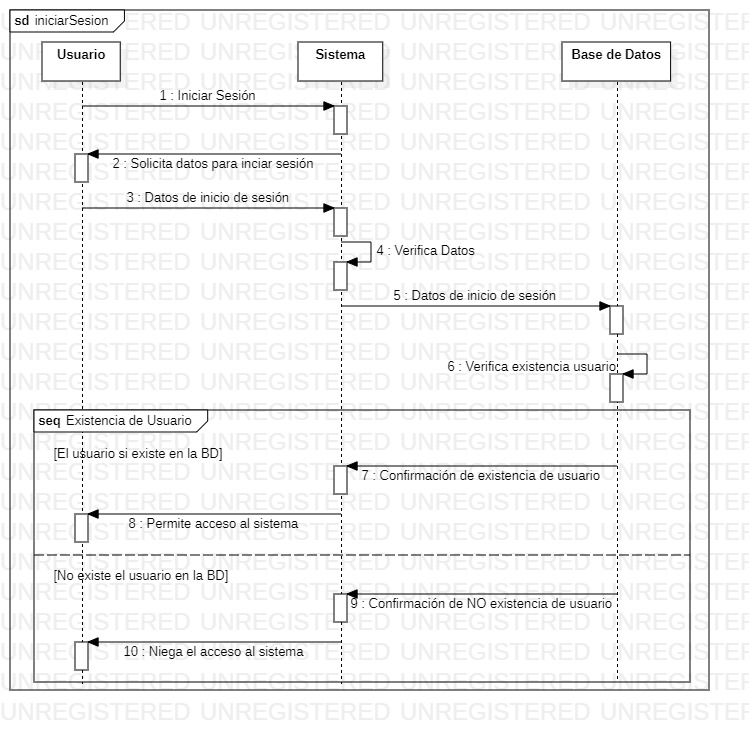
\includegraphics[width=1\textwidth]{./diseno/vprocesos/imagenes/iniciarSesion}
	\caption{Diagrama de Secuencia - Iniciar Sesión}
	\label{fig:Diagrama de Secuencia - Iniciar Sesión}
\end{figure}
\clearpage
\subsection{Visualizar Menú}
En la figura \ref{fig:Diagrama de Secuencia - Visualizar Menú} mostramos el diagrama de secuencia correspondiente a la función de visualizar menú, aquí el Mecánico (usuario) puede elegir dos opciones:
\begin{itemize}
	\item \textbf{Gestión de Agenda:} Al elegir esta opción, el usuario podrá entrar a otra parte del sistema para que pueda interactuar con la base de datos mediante una interfaz gráfica. Es decir, que llevará a cabo las diversas tareas para poder tener un control sobre la información a cerca de los vehículos a reparar.
	\item \textbf{Gestión de Refacciones:} Si el usuario elige esta opción, el usuario podrá visualizar las refacciones que existen en el almacén del taller. En caso de que no exista la pieza que el necesita, podrá generar una solicitud dentro del mismo sistema. 
\end{itemize}
\begin{figure}[!h]
	\centering
	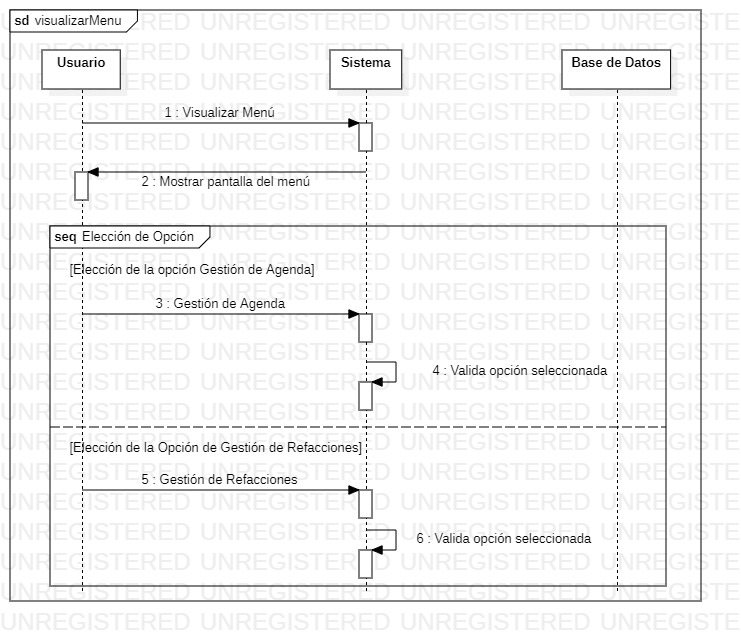
\includegraphics[width=0.9\textwidth]{./diseno/vprocesos/imagenes/visualizarMenu}
	\caption{Diagrama de Secuencia - Visualizar Menú}
	\label{fig:Diagrama de Secuencia - Visualizar Menú}
\end{figure}
%Documentación de los vehículos
\subsection{Visualizar Agenda}
En la siguiente figura \ref{fig:Diagrama de Secuencia - Visualizar Agenda} se muestra el diagrama de secuencia que corresponde a la visualización de la agenda que el Mecánico (Usuario) tiene en cuanto a los vehículos que va a reparar dentro del taller. Existen dos posibilidades dentro de esta actividad:
\begin{itemize}
	\item \textbf{Si existen registros:} Al momento de que el usuario entra a esta parte del sistema, al existir registros de vehículos por reparar, se muestra toda la información en una tabla y/o lista para su posterior gestión.  
	\item \textbf{No existen registros:} No hay vehículos registrados por reparar, se muestra una tabla y/o lista vacía en pantalla.
\end{itemize}
\begin{figure}[!h]
	\centering
	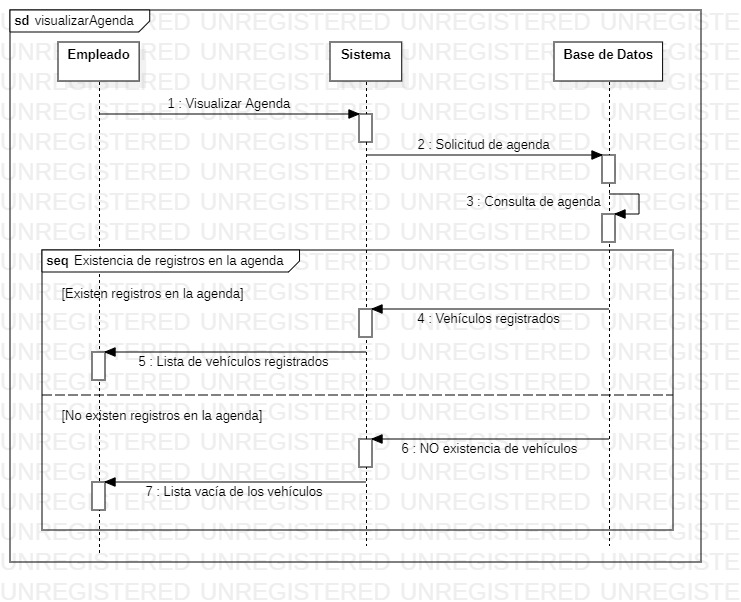
\includegraphics[width=1\textwidth]{./diseno/vprocesos/imagenes/visualizarAgenda}
	\caption{Diagrama de Secuencia - Visualizar Agenda}
	\label{fig:Diagrama de Secuencia - Visualizar Agenda}
\end{figure}
\subsubsection{Registrar Entrada de Vehículo}
En la figura \ref{fig:Diagrama de Secuencia - Registrar Entrada de Vehículo} se plasma el diagrama de secuencia que corresponde al registro de entrada de un vehículo al taller. El Mecánico (usuario) solicitará esta opción al sistema y este mismo le solicitará por medio de un formulario los datos necesarios para hacer el registro en la base de datos. Hay dos variantes en cuanto a la información ingresada: 
\begin{itemize}
	\item \textbf{Información válida:} Los datos que ha ingresado el usuario son válidos, es decir, que todos los campos han sido llenados y el formato del campo ingresado es el correcto. 
	\item \textbf{Información no válida:} Los datos que ha ingresado el usuario no son correctos. 
\end{itemize}
\begin{figure}[!h]
	\centering
	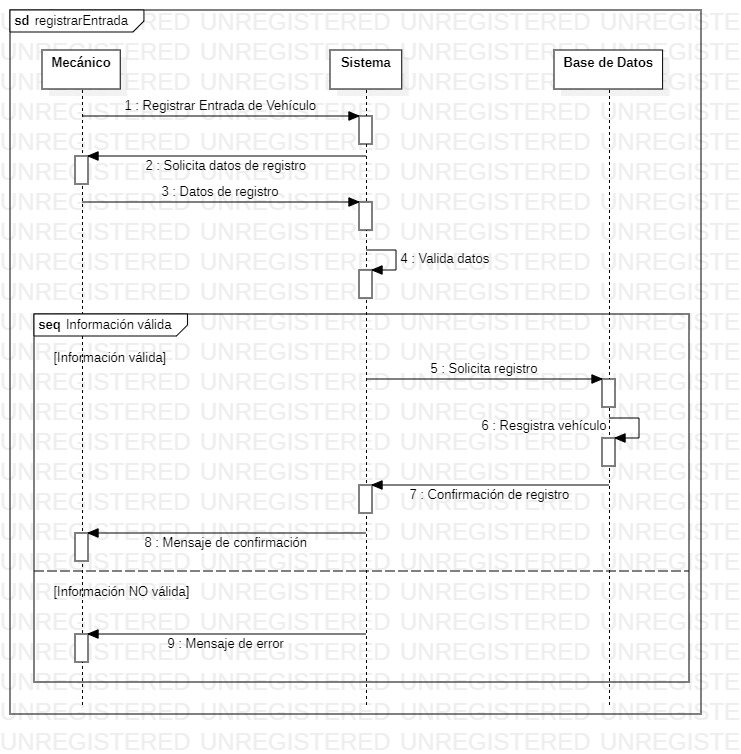
\includegraphics[width=0.8\textwidth]{./diseno/vprocesos/imagenes/registrarEntrada}
	\caption{Diagrama de Secuencia - Registrar Entrada de Vehículo}
	\label{fig:Diagrama de Secuencia - Registrar Entrada de Vehículo}
\end{figure}
\subsection{Modificar Entrada de Vehículo}
En la figura \ref{fig:Diagrama de Secuencia - Modificar Entrada de Vehículo} que se muestra a continuación se muestra el flujo de las diversas actividades que corresponden a la modificación de los datos de un registro de un vehículo. En este proceso, el usuario solicita esta modificación a través del sistema y este mismo interactúa con la base de datos para su modificación. En este proceso existen algunas variantes:
\begin{itemize}
	\item \textbf{Existe de vehículo:} Se corrobora que el vehículo está registrado en la base de datos, si es así, se procede a la modificación del mismo mediante un formulario de actualización.
	\item \textbf{No existe el vehículo:} Si no existe el vehículo en la base de datos, el sistema muestra un mensaje de error al usuario.
	\item \textbf{Datos válidos:} Al modificar los datos de un vehículo, el sistema valida si esa información es correcta, es decir, si los campos han sido llenados y el formato es el correspondiente con cada uno de dichos campos.
	\item \textbf{Datos no válidos:} Los datos que se quieren sobrescribir en la base de datos son incorrectos y el sistema no permite la actualización y muestra un mensaje de error.
\end{itemize}
\begin{figure}[!h]
	\centering
	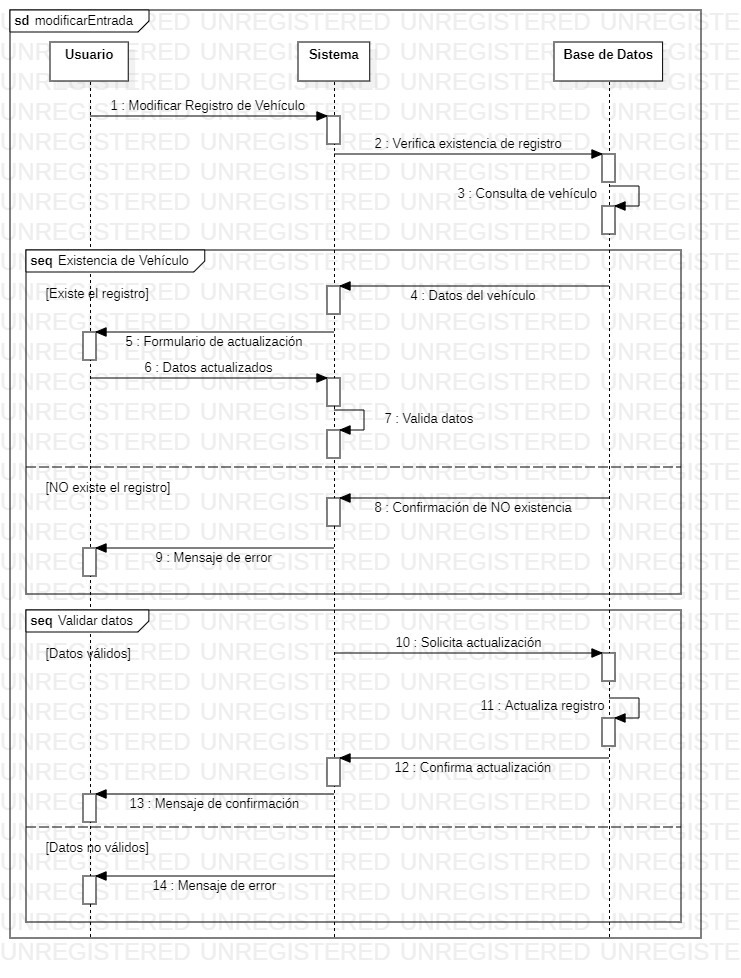
\includegraphics[width=1\textwidth]{./diseno/vprocesos/imagenes/modificarEntrada}
	\caption{Diagrama de Secuencia - Modificar Entrada de Vehículo}
	\label{fig:Diagrama de Secuencia - Modificar Entrada de Vehículo}
\end{figure}
\clearpage
\subsection{Eliminar Registro de Vehículo}
En la siguiente imagen \ref{fig:Diagrama de Secuencia - Eliminar Entrada de Vehículo}, se muestra el diagrama de secuencia correspondiente a la eliminación de algún registro para darle 'salida' al vehículo que se ha reparado. El sistema muestra un 'mensaje de seguridad' para verificar al usuario si esta seguro de borrar ese registro de la base de datos. Es en este punto donde el sistema toma dos caminos:
\begin{itemize}
	\item \textbf{Aceptación:} El Mecánico (usuario) acepta que desea eliminar ese registro, el sistema solicita a la base de datos la eliminación de dicho registro.
	\item \textbf{Cancelación:} Se elige la opción 'Cancelar' en la interfaz de usuario, el sistema desaparece el 'mensaje de seguridad' y la base de datos queda intacta. 
\end{itemize}
\begin{figure}[!h]
	\centering
	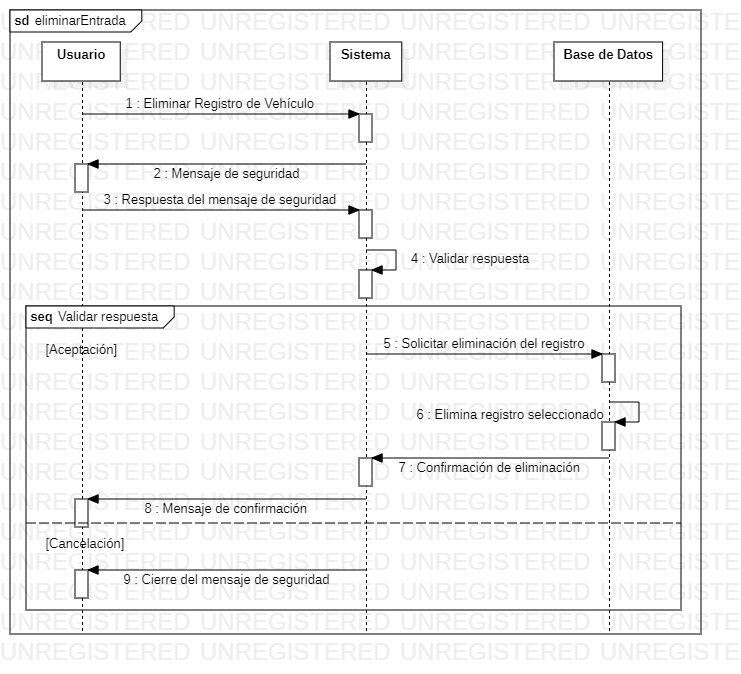
\includegraphics[width=0.9\textwidth]{./diseno/vprocesos/imagenes/eliminarEntrada}
	\caption{Diagrama de Secuencia - Eliminar Entrada de Vehículo}
	\label{fig:Diagrama de Secuencia - Eliminar Entrada de Vehículo}
\end{figure}
\clearpage
\subsection{Buscar Registro de Vehículo}
En la siguiente figura, la \ref{fig:Diagrama de Secuencia - Eliminar Entrada de Vehículo}, corresponde al diagrama de secuencia a la actividad de buscar algún registro de vehículo en específico, esto para ahorrar un poco más de tiempo en la búsqueda de ducho registro. Existen dos variantes en este proceso:
\begin{itemize}
	\item \textbf{Existe el registro:} Al encontrar el registro en la base de datos, se muestra en pantalla y se podrá interactuar con estos datos.
	\item \textbf{No existe el registro:} Si no se encuentra el registro, se mostrará en pantalla una lista y/o tabla en pantalla.
\end{itemize}
\begin{figure}[!h]
	\centering
	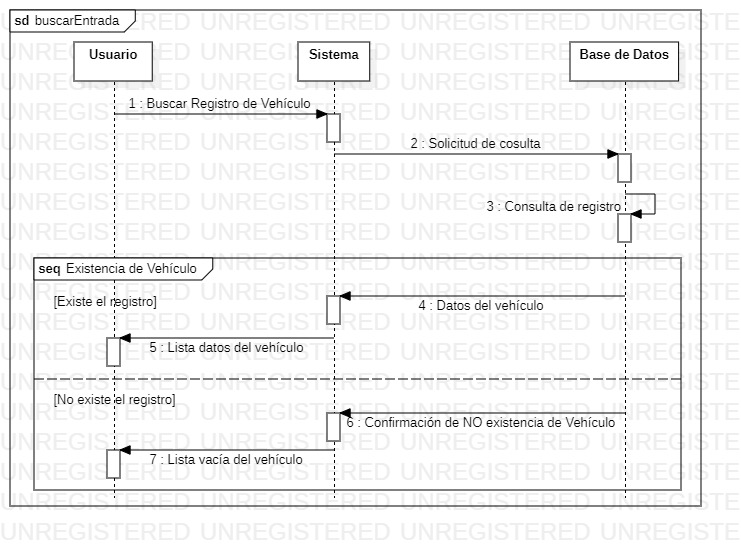
\includegraphics[width=1\textwidth]{./diseno/vprocesos/imagenes/buscarEntrada}
	\caption{Diagrama de Secuencia - Buscar Entrada de Vehículo}
	\label{fig:Diagrama de Secuencia - Buscar Entrada de Vehículo}
\end{figure}
 \clearpage
\subsubsection{Visualizar Refacciones Disponibles}
En la figura \ref{fig:Diagrama de Secuencia - Visualizar Refacciones} se muestra el diagrama de proceso que corresponde a la visualización de las refacciones que se encuentran en el almacén del taller. La aplicación hace la consulta a la base de datos y es aquí donde el software puede tomar dos opciones: 
\begin{itemize}
	\item \textbf{Existen registros:} Hay refacciones en almacenes, y se puede seleccionar alguna de ellas para implementarla en la reparación de un vehículo registrado.
	\item \textbf{No existen registros:} La base de datos manda un mensaje para la aplicación, la cual le muestra al Mecánico (usuario) una lista y/o tabla vacía. 
\end{itemize} 
\begin{figure}[!h]
	\centering
	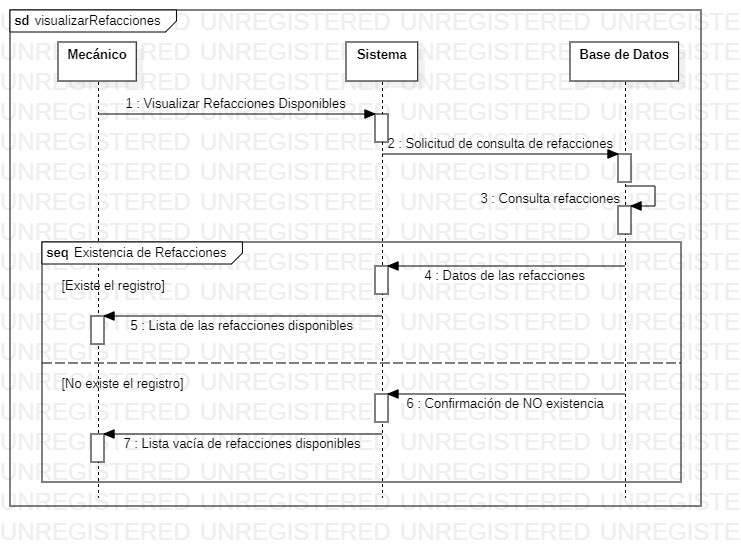
\includegraphics[width=1\textwidth]{./diseno/vprocesos/imagenes/visualizarRefacciones}
	\caption{Diagrama de Secuencia - Visualizar Refacciones}
	\label{fig:Diagrama de Secuencia - Visualizar Refacciones}
\end{figure}
\subsubsection{Solicitar Refacción}
En la siguiente figura \ref{fig:Diagrama de Secuencia - Solicitar Refaccion} se muestran la secuencia de las actividades que se deben de llevar a cabo para realizar la solicitud de una refacción que no se encuentre en el almacén del taller. El sistema solicita información al Mecánico (usuario) para generar una solicitud. Al ingresar datos al sistema, existe una validación de estos mismos datos, esto lleva al sistema a tomar dos caminos: 
\begin{itemize}
	\item \textbf{Información válida:} Los datos ingresados por el usuario son válidos, el formato y los campos han sido llenados correctamente de acuerdo a los datos que el sistema solicite.  
	\item \textbf{Información no válida:} Los datos ingresados por el usuario no son válidos, los campos o el formato no son correctos y el sistema muestra un mensaje de error.
\end{itemize} 
\begin{figure}[!h]
	\centering
	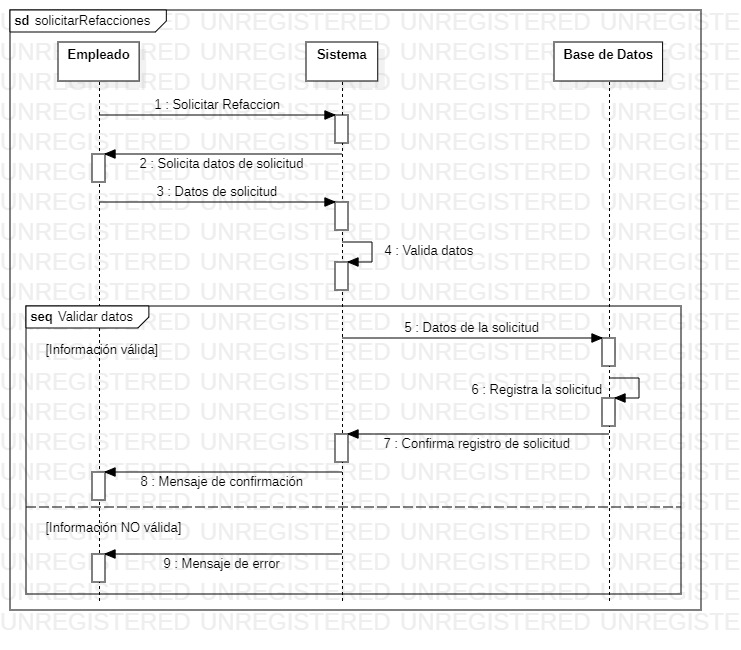
\includegraphics[width=0.9\textwidth]{./diseno/vprocesos/imagenes/solicitarRefacciones}
	\caption{Diagrama de Secuencia - Solicitar Refacción}
	\label{fig:Diagrama de Secuencia - Solicitar Refaccion}
\end{figure}
\clearpage
\subsection{Vista de Procesos Administrador}
El administrador también tiene poder sobre la gestión de los vehículos que entran al taller. Dicho poder lo comparte con el empleado, para visualizar mas a detalle estos procesos vea la sección de 'Vista de Procesos Empleado' \ref{subsec: Vista Procesos Empleado}.
%Documetnación de los empleados
\subsubsection{Visualizar Empleados}
En la siguiente figura \ref{fig:Diagrama de Secuencia - Visualizar Agenda} se muestra el diagrama de secuencia que corresponde a la visualización de cada uno de los registros de los empleados que existen dentro de la base de datos, existen dos posibilidades dentro de esta actividad:
\begin{itemize}
	\item \textbf{Si existen registros:} Al momento de que el administrador entra a esta parte del sistema, al existir registros de empleados, se muestra toda la información en una tabla y/o lista para su posterior gestión.  
	\item \textbf{No existen registros:} No hay empleados registrados, se muestra una tabla y/o lista vacía en pantalla.
\end{itemize}
\begin{figure}[!h]
	\centering
	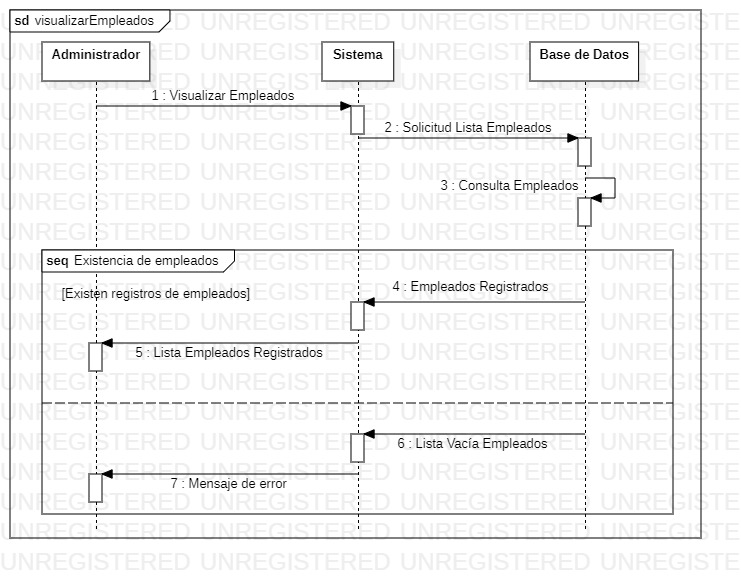
\includegraphics[width=0.8\textwidth]{./diseno/vprocesos/imagenes/visualizarEmpleados}
	\caption{Diagrama de Secuencia - Visualizar Empleados}
	\label{fig:Diagrama de Secuencia - Visualizar Empleados}
\end{figure}
\subsubsection{Registrar Nuevo Empleado}
En la figura \ref{fig:Diagrama de Secuencia - Registrar Nuevo Empleado} se plasma el diagrama de secuencia que corresponde al registro de un nuevo empleado dentro de la base de datos. El administrador solicitará esta opción al sistema y este mismo le solicitará por medio de un formulario los datos necesarios para hacer el registro en la base de datos. Hay dos variantes en cuanto a la información ingresada: 
\begin{itemize}
	\item \textbf{Información válida:} Los datos que ha ingresado el administrador son válidos, es decir, que todos los campos han sido llenados y el formato del campo ingresado es el correcto. 
	\item \textbf{Información no válida:} Los datos que ha ingresado el usuario no son correctos. 
\end{itemize}
\begin{figure}[!h]
	\centering
	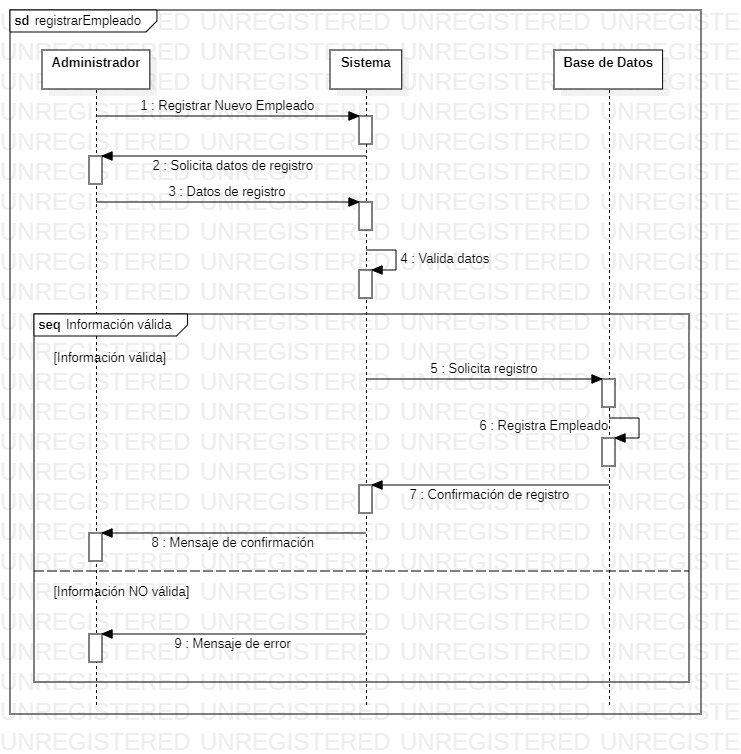
\includegraphics[width=0.8\textwidth]{./diseno/vprocesos/imagenes/registrarEmpleado}
	\caption{Diagrama de Secuencia - Registrar Nuevo Empleado}
	\label{fig:Diagrama de Secuencia - Registrar Nuevo Empleado}
\end{figure}
\subsubsection{Modificar Empleado}
En la figura \ref{fig:Diagrama de Secuencia - Modificar Empleado} que se muestra a continuación se muestra el flujo de las diversas actividades que corresponden a la modificación de los datos de un registro de un empleado. En este proceso, el administrador solicita esta modificación a través del sistema y este mismo interactúa con la base de datos para su modificación. En este proceso existen algunas variantes:
\begin{itemize}
	\item \textbf{Existe empleado:} Se asegura que el empleado está registrado en la base de datos, si es así, se procede a la modificación del mismo mediante un formulario de actualización.
	\item \textbf{No existe el empleado:} Si no existe el registro del empleado en la base de datos, el sistema muestra un mensaje de error al usuario.
	\item \textbf{Datos válidos:} Al modificar los datos de un empleado, el sistema valida si esa información es correcta, es decir, si los campos han sido llenados y el formato es el correspondiente con cada uno de dichos campos.
	\item \textbf{Datos no válidos:} Los datos que se quieren sobrescribir en la base de datos son incorrectos y el sistema no permite la actualización y muestra un mensaje de error.
\end{itemize}
\begin{figure}[!h]
	\centering
	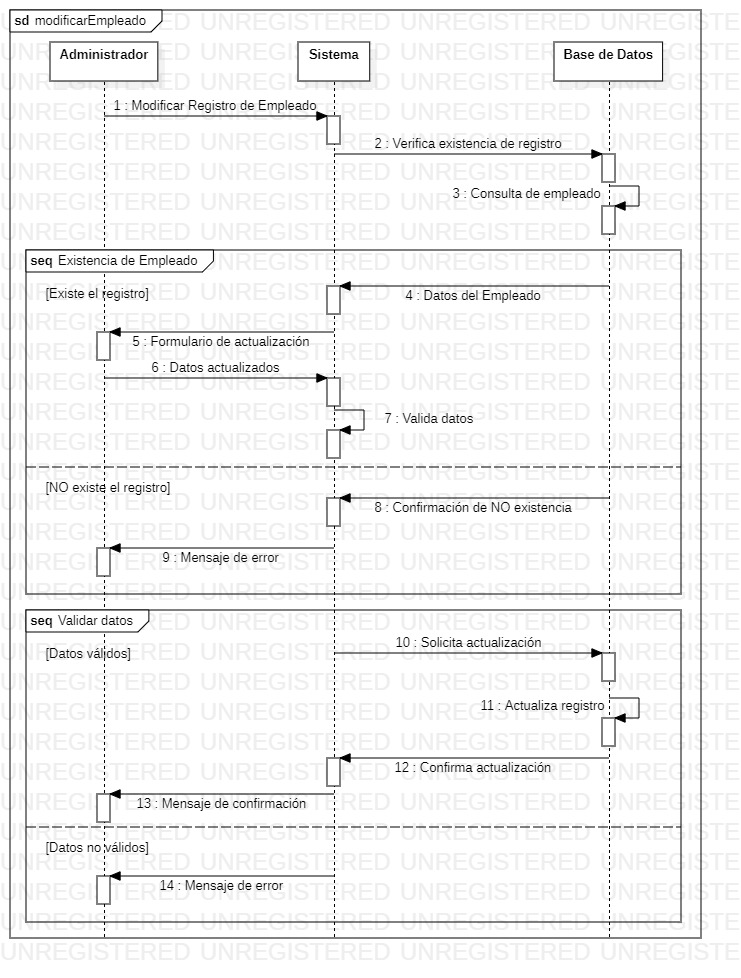
\includegraphics[width=1\textwidth]{./diseno/vprocesos/imagenes/modificarEmpleado}
	\caption{Diagrama de Secuencia - Modificar Empleado}
	\label{fig:Diagrama de Secuencia - Modificar Empleado}
\end{figure}
\clearpage
\subsubsection{Eliminar Empleado}
En la siguiente imagen \ref{fig:Diagrama de Secuencia - Eliminar Empleado}, se muestra el diagrama de secuencia correspondiente a la eliminación de algún registro de un empleado, esto en el caso de que ya no pertenezca a la organización o simplemente renunció. El sistema muestra un 'mensaje de seguridad' para verificar al administrador si esta seguro de borrar ese registro de la base de datos. Existen dos posibilidades dentro de este módulo:
\begin{itemize}
	\item \textbf{Aceptación:} El administrador acepta que desea eliminar ese registro, el sistema solicita a la base de datos la eliminación de dicho registro y se muestra un mensaje de que el empleado ha sido eliminado de manera satisfactoria.
	\item \textbf{Cancelación:} Si elige la opción 'Cancelar' en la interfaz de usuario, el sistema desaparece el 'mensaje de seguridad' y la base de datos queda intacta. 
\end{itemize}
\begin{figure}[!h]
	\centering
	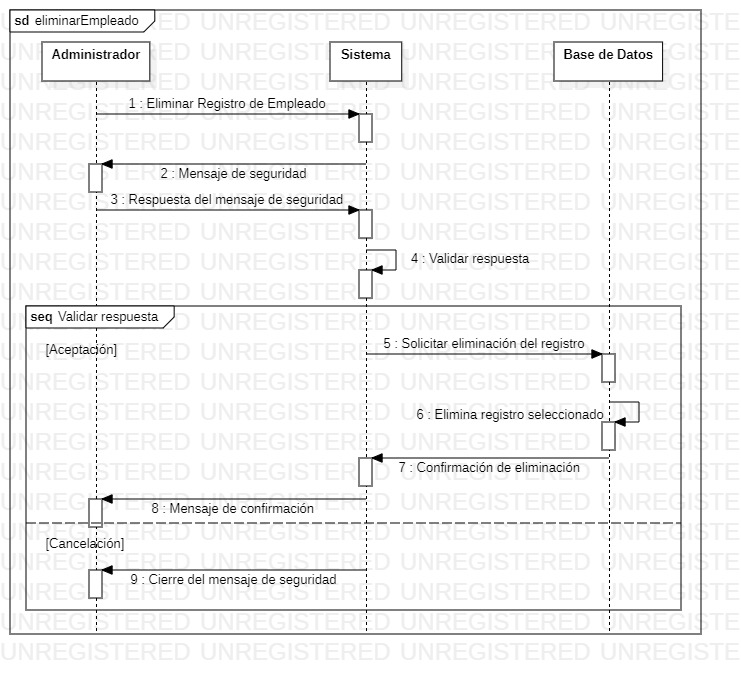
\includegraphics[width=0.8\textwidth]{./diseno/vprocesos/imagenes/eliminarEmpleado}
	\caption{Diagrama de Secuencia - Eliminar Empleado}
	\label{fig:Diagrama de Secuencia - Eliminar Empleado}
\end{figure}
\clearpage
\subsubsection{Buscar Registro de Vehículo}
En el siguiente diagrama, la \ref{fig:Diagrama de Secuencia - Eliminar Entrada de Vehículo}, corresponde la secuencia de actividades para buscar algún registro de un empleado en específico, esto para ahorrar un poco más de tiempo en la búsqueda de ducho registro y poder realizar alguna acción sobre ese registro. Existen dos variantes en este proceso:
\begin{itemize}
	\item \textbf{Existe el registro:} Al encontrar el registro en la base de datos, se muestra en pantalla y se podrá interactuar con estos datos.
	\item \textbf{No existe el registro:} Si no se encuentra el registro, se mostrará en pantalla una lista y/o tabla en pantalla.
\end{itemize}
\begin{figure}[!h]
	\centering
	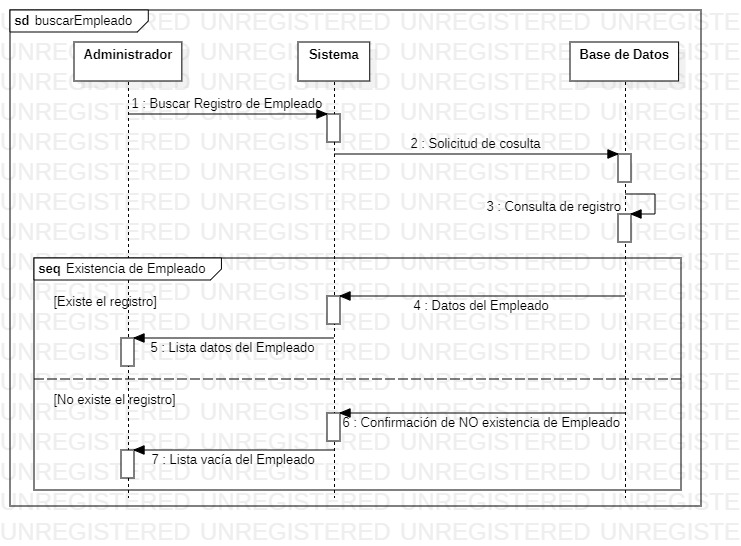
\includegraphics[width=1\textwidth]{./diseno/vprocesos/imagenes/buscarEmpleado}
	\caption{Diagrama de Secuencia - Buscar Empleado}
	\label{fig:Diagrama de Secuencia - Buscar Empleado}
\end{figure}
\clearpage
%Documentación de las refacciones
\subsubsection{Registrar Refacción}
En la siguiente figura \ref{fig:Diagrama de Secuencia - Registrar Refaccion} se muestra el diagrama de secuencia que corresponde al registro de una refacción que vaya a entrar al almacén, esta puede haber sido solicitada por un empleado o no. El administrador solicitará esta opción al sistema y este mismo le solicitará por medio de un formulario los datos necesarios para hacer el registro en la base de datos. Hay dos variantes en cuanto a la información ingresada: 
\begin{itemize}
	\item \textbf{Información válida:} Los datos que ha ingresado el administrador son válidos, es decir, que todos los campos han sido llenados y el formato del campo ingresado es el correcto. 
	\item \textbf{Información no válida:} Los datos que ha ingresado el usuario no son correctos. 
\end{itemize}
\begin{figure}[!h]
	\centering
	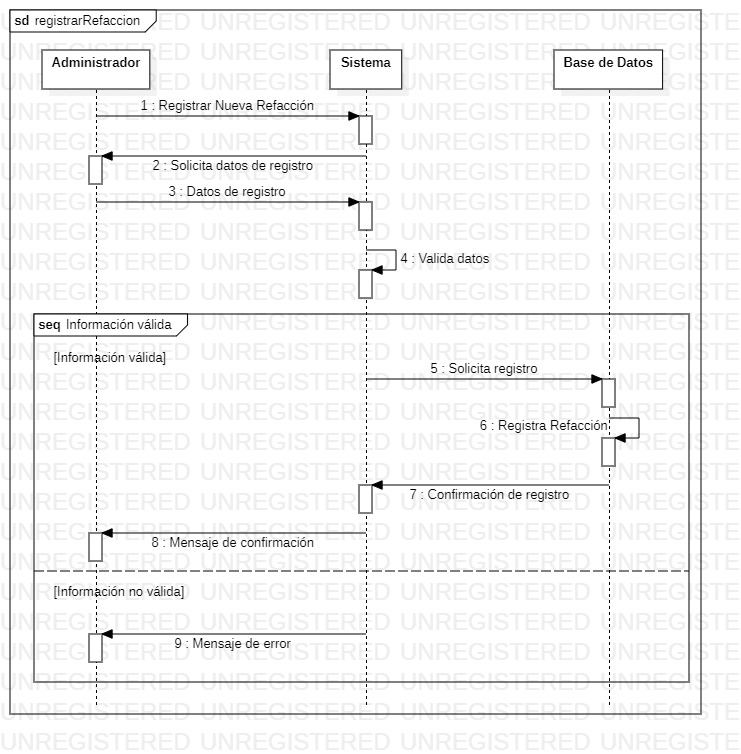
\includegraphics[width=0.8\textwidth]{./diseno/vprocesos/imagenes/registrarRefaccion}
	\caption{Diagrama de Secuencia - Registrar Refacción}
	\label{fig:Diagrama de Secuencia - Registrar Refaccion}
\end{figure}
\subsubsection{Modificar Refacción}
En la figura \ref{fig:Diagrama de Secuencia - Modificar Empleado} se muestra el flujo de las diversas actividades que corresponden a la modificación de los datos de una refacción que se encuentra en almacén del taller, esto en dado caso que haya un error en la captura de dichos datos. En este proceso, el administrador solicita esta modificación a través del sistema y este mismo interactúa con la base de datos para su modificación. En este proceso existen tres variantes para los datos a modificar:
\begin{itemize}
	\item \textbf{Existe empleado:} Se asegura que la refacción está registrada,en dado caso que si, se procede a la modificación del mismo mediante un formulario de actualización.
	\item \textbf{No existe el empleado:} Si no existe el registro de la refacción en la base de datos, el sistema muestra un mensaje de error al usuario.
	\item \textbf{Datos válidos:} Al modificar los datos de un empleado, el sistema valida si esa información es correcta, es decir, si los campos han sido llenados y el formato es el correspondiente con cada uno de dichos campos.
	\item \textbf{Datos no válidos:} Los datos que se quieren sobrescribir en la base de datos son incorrectos y el sistema no permite la actualización y muestra un mensaje de error.
\end{itemize}
\begin{figure}[!h]
	\centering
	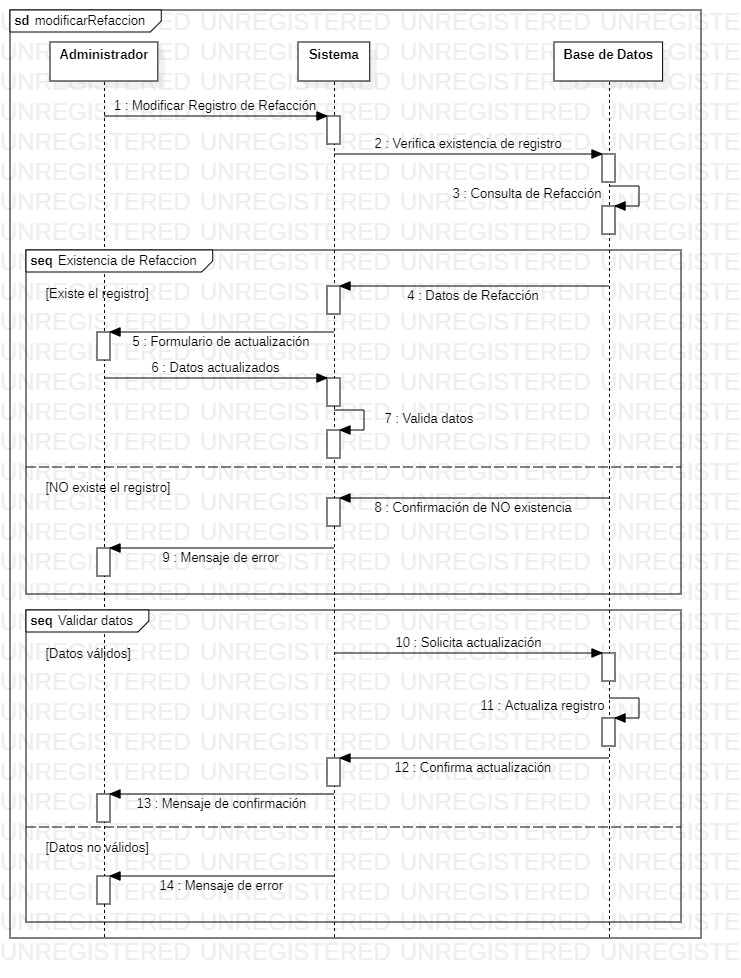
\includegraphics[width=1\textwidth]{./diseno/vprocesos/imagenes/modificarRefaccion}
	\caption{Diagrama de Secuencia - Modificar Refacción}
	\label{fig:Diagrama de Secuencia - Modificar Refaccion}
\end{figure}
\clearpage
\subsubsection{Eliminar Refaccion}
En la siguiente imagen \ref{fig:Diagrama de Secuencia - Eliminar Refaccion}, se muestra el diagrama de secuencia correspondiente a la eliminación de algún registro de una refacción que estaba en alamcén del taller, esto en el caso de que ya no haya en existencia o el proveedor no las haya conseguido. El sistema muestra un 'mensaje de seguridad' para verificar al administrador si esta seguro de borrar ese registro de la base de datos. Existen dos posibilidades dentro de este módulo:
\begin{itemize}
	\item \textbf{Aceptación:} El administrador acepta que desea eliminar ese registro, el sistema solicita a la base de datos la eliminación de dicho registro y se muestra un mensaje de que el empleado ha sido eliminado de manera satisfactoria.
	\item \textbf{Cancelación:} Si elige la opción 'Cancelar' en la interfaz de usuario, el sistema desaparece el 'mensaje de seguridad' y la base de datos queda intacta. 
\end{itemize}
\begin{figure}[!h]
	\centering
	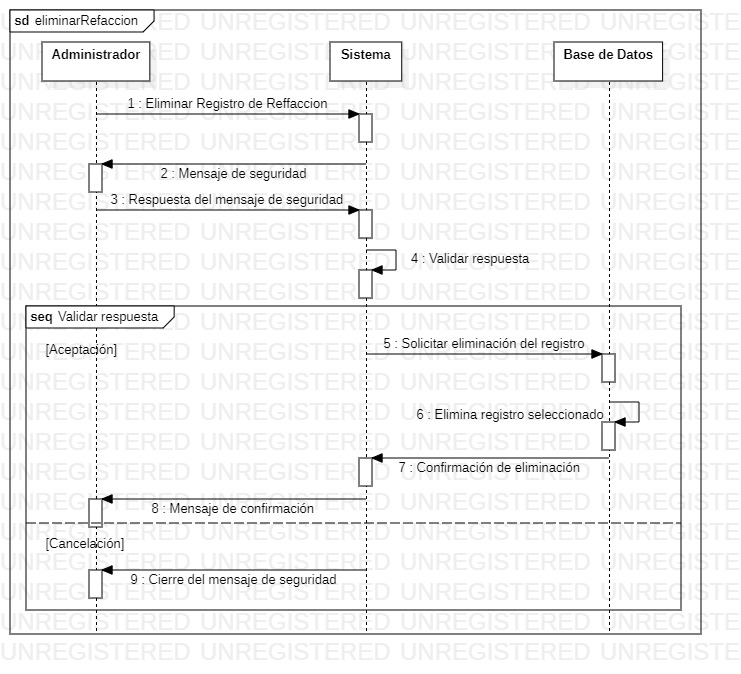
\includegraphics[width=0.8\textwidth]{./diseno/vprocesos/imagenes/eliminarRefaccion}
	\caption{Diagrama de Secuencia - Eliminar Refacción}
	\label{fig:Diagrama de Secuencia - Eliminar Refaccion}
\end{figure}
\clearpage
\subsubsection{Buscar Refacción}
En el siguiente diagrama, la \ref{fig:Diagrama de Secuencia - Eliminar Entrada de Vehículo}, corresponde la secuencia de actividades para buscar algún registro de un empleado en específico, esto para ahorrar un poco más de tiempo en la búsqueda de ducho registro y poder realizar alguna acción sobre ese registro. Existen dos variantes en este proceso:
\begin{itemize}
	\item \textbf{Existe el registro:} Al encontrar el registro en la base de datos, se muestra en pantalla y se podrá interactuar con estos datos.
	\item \textbf{No existe el registro:} Si no se encuentra el registro, se mostrará en pantalla una lista y/o tabla en pantalla.
\end{itemize}
\begin{figure}[!h]
	\centering
	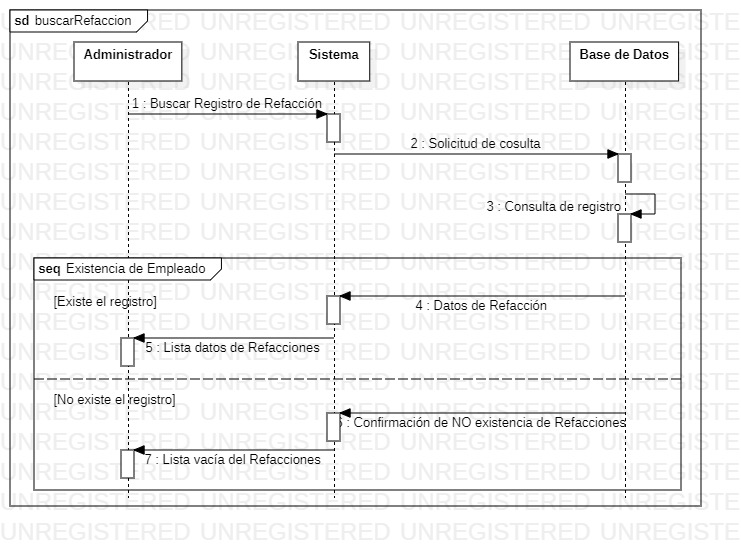
\includegraphics[width=1\textwidth]{./diseno/vprocesos/imagenes/buscarRefaccion}
	\caption{Diagrama de Secuencia - Buscar Refacción}
	\label{fig:Diagrama de Secuencia - Buscar Refaccion}
\end{figure}
\clearpage
%Documetnación de solicitudes
\subsubsection{Visualizar Solicitud}
En la siguiente figura \ref{fig:Diagrama de Secuencia - Visualizar Solicitudes de Refaccion} se muestra el diagrama de secuencia que corresponde a la visualización de todas las solicitudes que los diversos empleados han realizado para que puedan hacer su trabajo, existen dos posibilidades dentro de esta actividad:
\begin{itemize}
	\item \textbf{Si existen registros:} Al momento de que el administrador entra a esta parte del sistema, se muestra en una tabla y/o lista toda la información necesaria para atender a las solicitudes que se necesiten.  
	\item \textbf{No existen registros:} No hay empleados registrados, se muestra una tabla y/o lista vacía en pantalla.
\end{itemize}
\begin{figure}[!h]
	\centering
	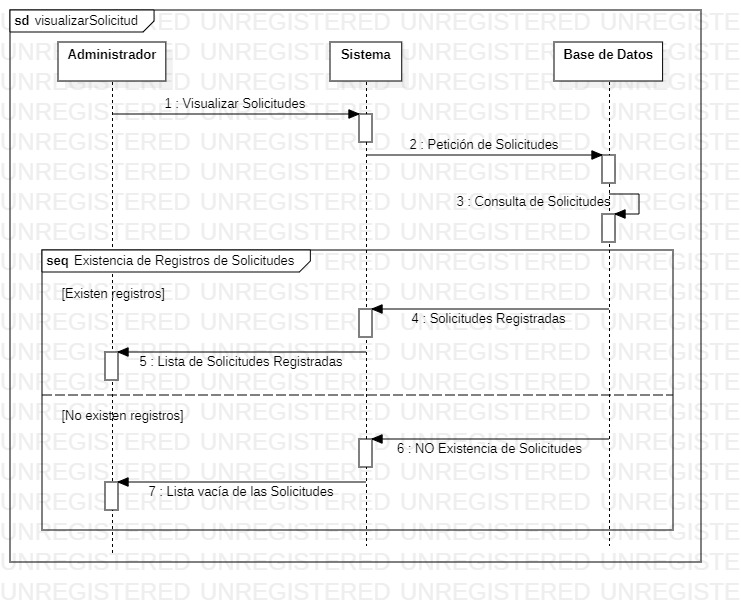
\includegraphics[width=0.8\textwidth]{./diseno/vprocesos/imagenes/visualizarSolicitud}
	\caption{Diagrama de Secuencia - Visualizar Solicitudes de Refacción}
	\label{fig:Diagrama de Secuencia - Visualizar Solicitudes de Refaccion}
\end{figure}
\clearpage
\subsubsection{Atender Solicitud}
En en siguiente diagrama\ref{fig:Diagrama de Secuencia - Visualizar Solicitudes de Refaccion} se muestra la secuencia que corresponde a la atención de todas las solicitudes que los diversos empleados han realizado para que puedan hacer su trabajo, al momento de aceptar la solicitud y atenderla el administrador ingresará unos datos que el sistema solicite, estos datos tendrán que ser verificados:
\begin{itemize}
	\item \textbf{Datos válidos:} Los datos ingresados por el administrador son correctos y cuentan con el formato específico para ser ingresados a la base de datos y atender a la solicitud del empleado.  
	\item \textbf{Datos no válidos} Los datos ingresados no son correctos o no cumplen con las especificaciones de formato.
\end{itemize}
\begin{figure}[!h]
	\centering
	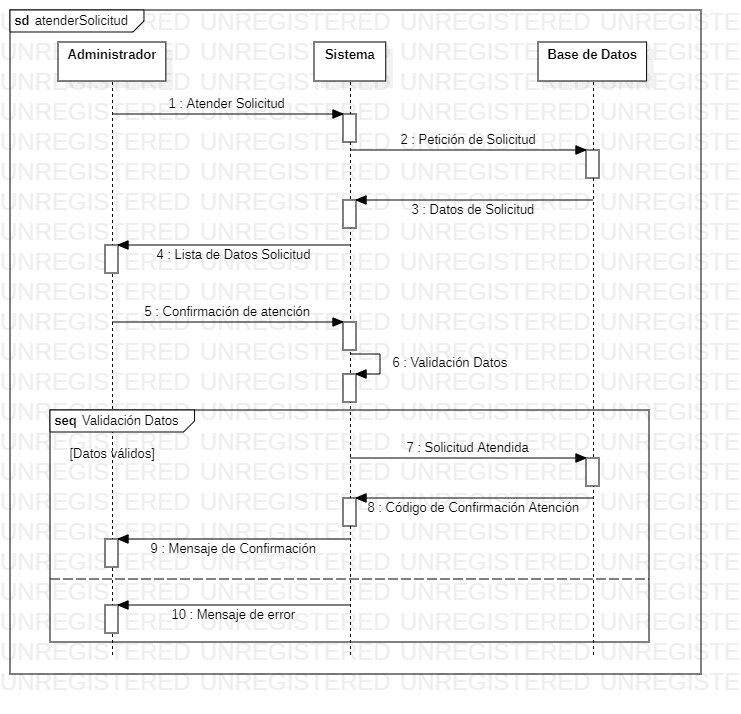
\includegraphics[width=0.8\textwidth]{./diseno/vprocesos/imagenes/atenderSolicitud}
	\caption{Diagrama de Secuencia - Atender Solicitud de Refacción}
	\label{fig:Diagrama de Secuencia - Atender Solicitud de Refaccion}
\end{figure}
\clearpage


\section{Vista Lógica}
En la figura \ref{fig:Diagrama de Clases - Vista Logica} se muestra un diagrama de clases que conforman la estructura de la base de datos para poder manipularla a través del sistema. Consta de 4 clases: Mecanico, Vehiculo, Refaccion, Solicitud. La clase Mecanico hereda de la clase Vehiculo que a su vez hereda de Refaccion y de Solicitud, esto para poder tener una relación entre todos los datos. En otras palabras, un Mecánico puede tener uno o varios Vehículos en el taller y estos mismos pueden necesitar una Refacción, estas a su vez pueden ser obtenidas mediante una Solicitud. 
Los atributos de cada clase son los siguientes: 
\begin{itemize}
	\item \textbf{Mecanico:}El nombre de usuario y contraseña.
	\item \textbf{Vehiculo:}El numero de inventario, la descripción del vehiculo (puede ser el modelo o señas particulares), la fecha de entrada y de salida además del procedimiento que se debe de realizar.
	\item \textbf{Refaccion:}El numero de inventario y la descripción de la refacción (para que vehículo funciona o señas particulares de la pieza).
	\item \textbf{Solicitud:}Identificador de la solicitud y fecha de la misma.
\end{itemize}
\begin{figure}[!h]
	\centering
	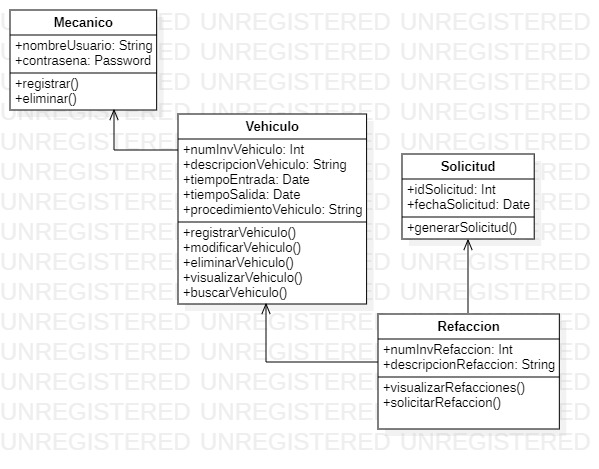
\includegraphics[width=1\textwidth]{./diseno/vlogica/imagenes/vistaLogica}
	\caption{Diagrama de Clases - Vista Lógica}
	\label{fig:Diagrama de Clases - Vista Logica}
\end{figure}
\clearpage
\section{Vista de Desarrollo}
En la siguiente figura \ref{fig:Diagrama de Componentes - Vista de Desarrollo} se muestra el diagrama de componentes del sistema, donde se muestran los diversos componentes e interfaces. Partimos de una principal, el IniciarSesion; por la cual se va a interactuar a la visualización del menú por medio de la pantallaMenu. Además este componente tiene una conexión a la base de datos para verificar la identidad del usuario y darle acceso o no al sistema. 
\\
Por medio del componente de VisualizarMenu, a través de la interfaz pantallaMenu, el usuario puede elegir una opción que el sistema ofrece. El componente de VisualizarAgenda tiene relación con los siguientes componentes e interfaces: 
\begin{itemize}
	\item \textbf{RegistrarVehiculo:} Por medio de la interfaz pantallaRegVehiculo, se tiene una conexión con este componente para el posterior registro en la base de datos.
	\item \textbf{ActualizarVehiculo:} Por medio de la interfaz pantallaActVehiculo, se tiene la conexión con este componente para poder modificar un registro de la base de datos.
	\item \textbf{EliminarVehiculo:} Por medio de la interfaz pantallaElimVehiculo, se tiene conexión con este componente para poder eliminar un registro de un vehículo.
	\item \textbf{BuscarVehiculo:} A través de la interfaz pantallaBusVehiculo, se tiene conexión con este componente para poder buscar un registro de un vehículo en especifico. 
\end{itemize}
Por otro lado, se tiene el componente VisualizarRefacciones, con el cual se obtiene una conexión por medio de la interfaz pantallaGestRef. Que a su vez, se conecta al componente RegistrarSolicitud por medio de la interfaz pantallaRegSol. Esto con la finalidad de visualizar si existen refacciones en almacén del taller o solicitar alguna. 
\begin{figure}[!h]
	\centering
	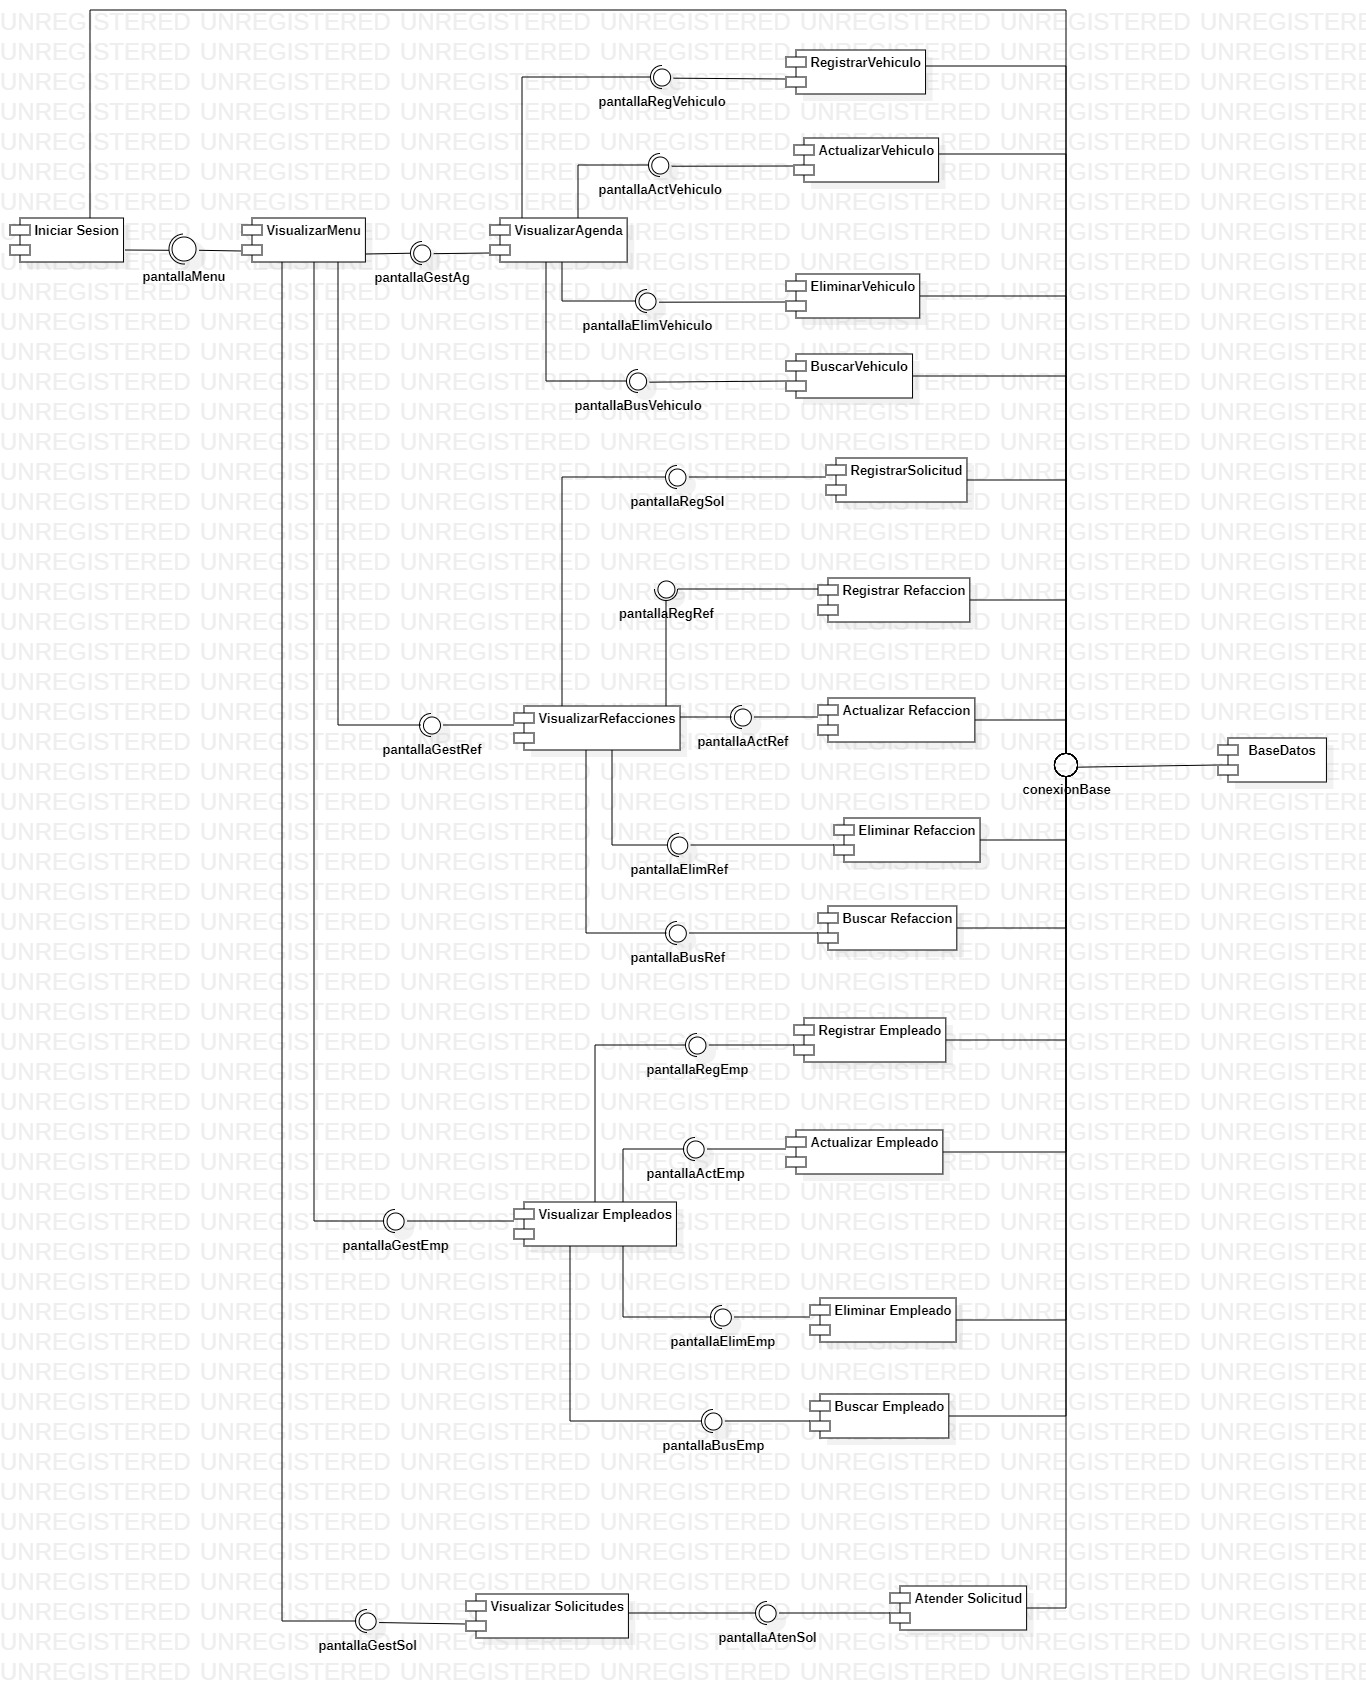
\includegraphics[width=1.3\textwidth]{./diseno/vdesarrollo/imagenes/vistaDesarrollo}
	\caption{Diagrama de Componentes - Vista de Desarrollo}
	\label{fig:Diagrama de Componentes - Vista de Desarrollo}
\end{figure}
\clearpage
\section{Vista Física}
En la siguiente imagen \ref{fig:Diagrama de Despliegue - Vista Física}, se muestra el diagrama de despliegue de la aplicación. Se tienen dos nodos, el primero es la computadora personal ya sea de escritorio o una laptop con cualquier sistema operativo, la única condición es que tenga Java instalado en su última versión para poder ejecutar el fichero 'mantenimiento.jar'. Del lado del servidor, se corre la base de datos que será manipulada por medio del sistema. 
\\
Básicamente se esta siguiendo un Modelo Cliente - Servidor, en este modelo el Cliente realiza peticiones al servidor y se llevan a cabo todas las tareas que se han programado en el sistema. Por otro lado en el Servidor, se encarga de 'escuchar' las peticiones del Cliente para manipular la información almacenados en la base de datos. Además también se muestra un driagrama de red \ref{fig:Diagrama de Red - Posible Escenario} donde la base de datos está alojada en 000WebHost (gratuito) además de los equipos de computo que contienen el ejecutable del programa.
\begin{figure}[!h]
	\centering
	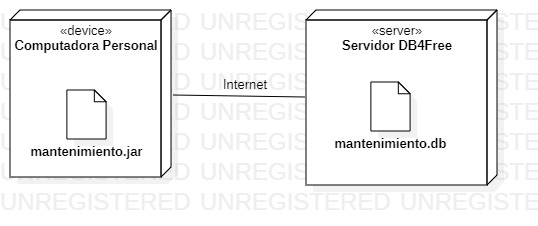
\includegraphics[width=0.9\textwidth]{./diseno/vfisica/imagenes/vistaFisica}
	\caption{Diagrama de Despliegue - Vista Física}
	\label{fig:Diagrama de Despliegue - Vista Física}
\end{figure}

\begin{figure}[!h]
	\centering
	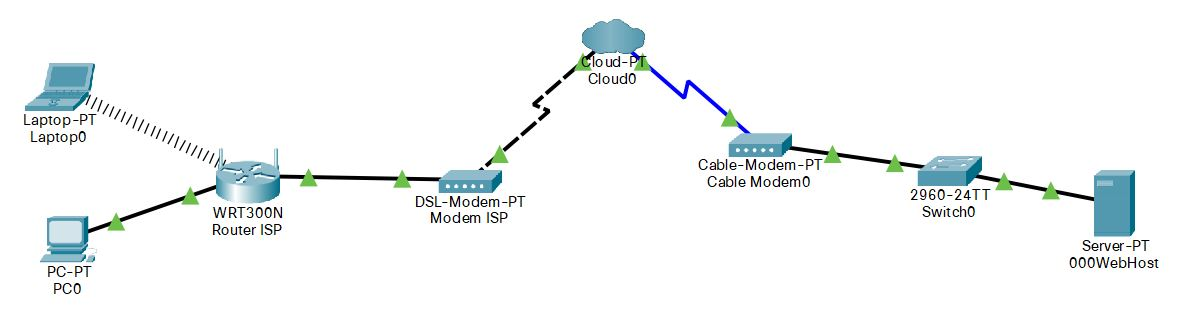
\includegraphics[width=0.9\textwidth]{./diseno/vfisica/imagenes/diagramaRed}
	\caption{Diagrama de Red - Posible Escenario}
	\label{fig:Diagrama de Red - Posible Escenario}
\end{figure}
\clearpage
\section{Vista de Escenarios}
En la siguiente figura, la \ref{fig:Diagrama de Casos de Uso - Vista de Escenarios}, se muestra la vista de escenarios representada por un diagrama de casos de uso. Este diagrama refleja los requerimientos funcionales principales del sistema. Cada caso de uso lo hemos identificado un una nomenclatura CU'X', siendo la letra 'X' el número del caso de uso al que se hace referencia.
\\
\begin{figure}[!h]
	\centering
	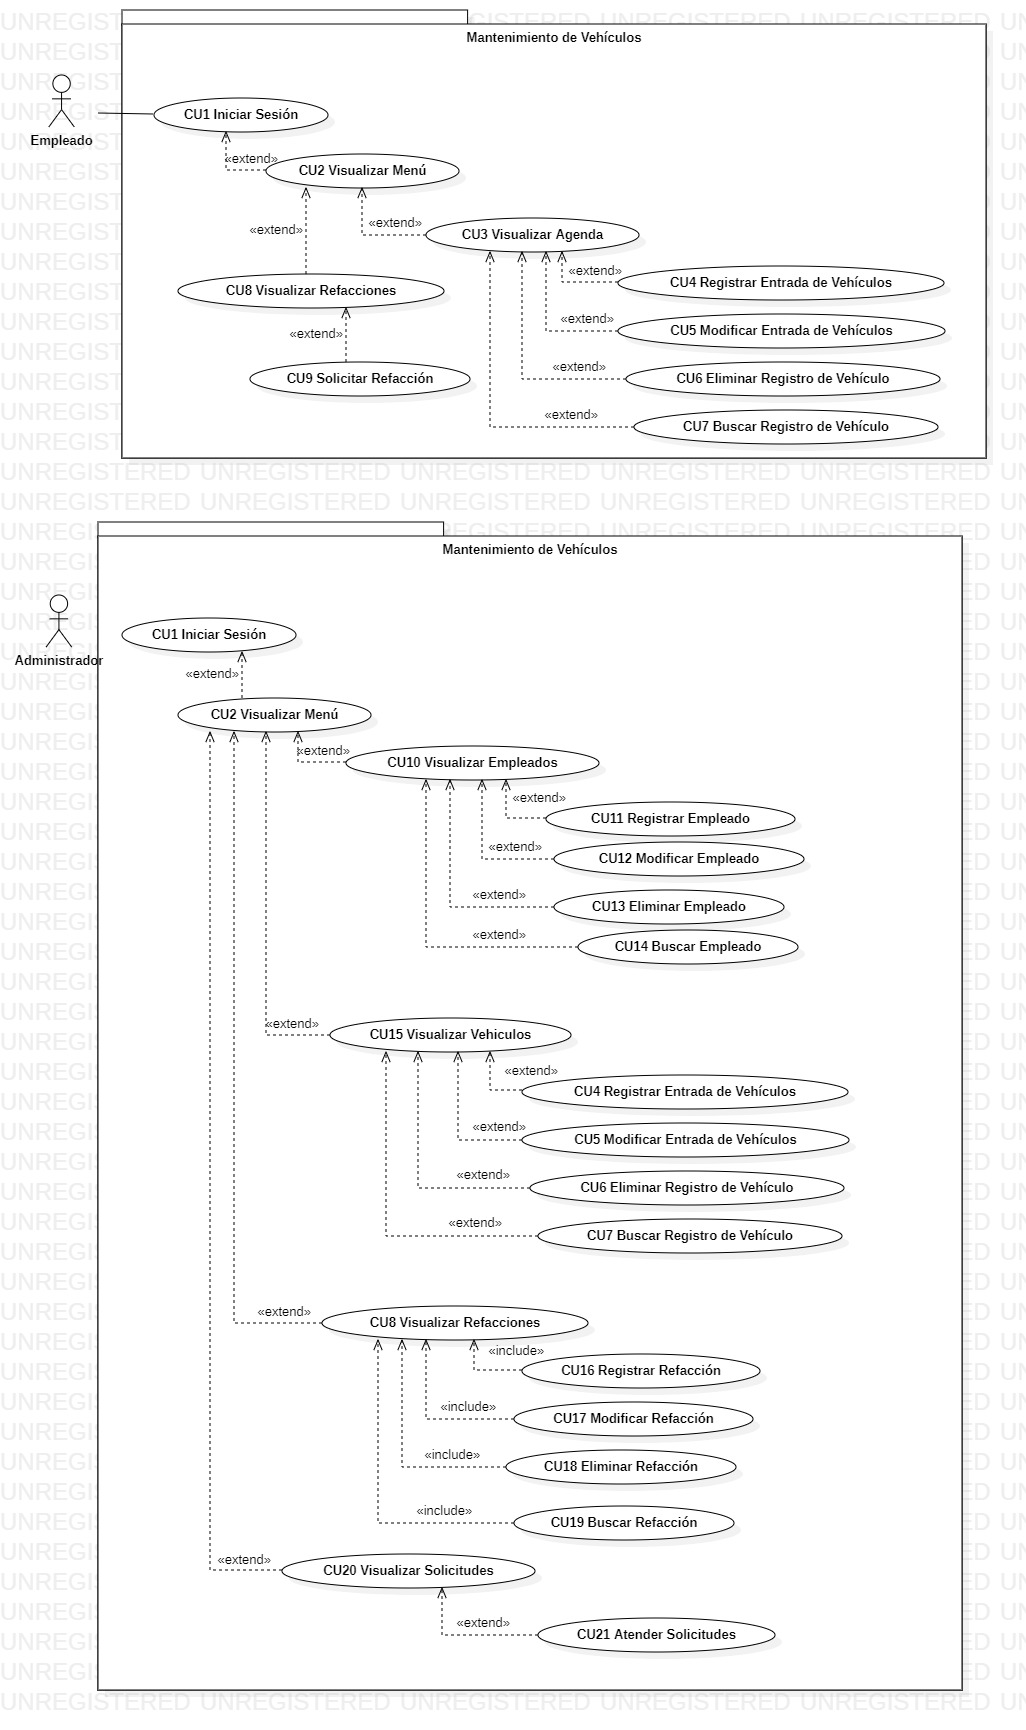
\includegraphics[width=1\textwidth]{./diseno/vescenarios/imagenes/vistaEscenarios}
	\caption{Diagrama de Casos de Uso - Vista de Escenarios}
	\label{fig:Diagrama de Casos de Uso - Vista de Escenarios}
\end{figure}
\\
A continuación se describen a detalle cada uno de los casos de uso que serán implementados en el sistema. Cada uno de estos casos también llevará un diseño de la UI (Interfaz de Usuario) para poder explicar el procedimiento de cada uno de los procesos. Cabe mencionar que estos casos de uso van de la mano con las historias de usuario descritas en el capítulo \ref{chap: historias de usuario}. 

\clearpage

%Contenido de la vista de escenarios
\subsection{CU1 Iniciar Sesión}
Esta pantalla (figura \ref{fig:Pantalla Iniciar Sesion - Vista de Escenarios}) será la primera en aparecer al ejecutarse el sistema. Se compone de un pequeño formulario donde el usuario (Mecánico) deberá teclear sus credenciales otorgadas por la administración de la empresa. Una vez ingresados de manera correcta, deberá pulsar el botón 'Ingresar'.
\\
En caso de que el usuario desee salir del sistema, solo deberá pulsar el botón 'Salir'. 
\\

\begin{figure}[!h]
	\centering
	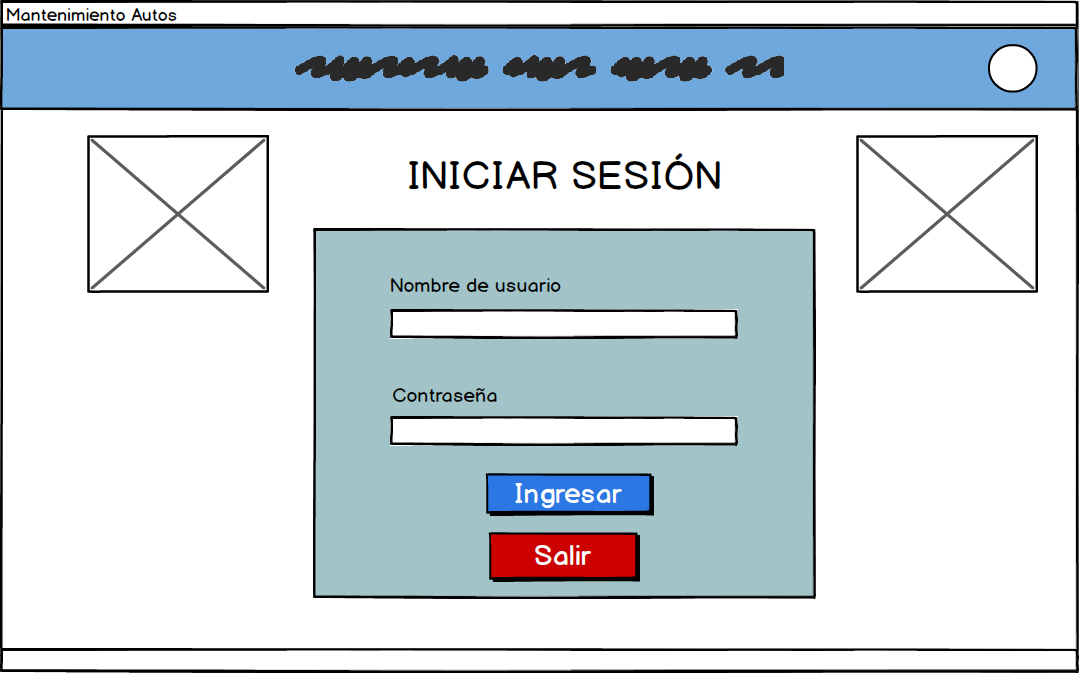
\includegraphics[width=1\textwidth]{./diseno/vescenarios/imagenes/Login}
	\caption{Pantalla Iniciar Sesión - Vista de Escenarios}
	\label{fig:Pantalla Iniciar Sesion - Vista de Escenarios}
\end{figure}
En ese sentido, si el usuario ingresa erróneamente sus credenciales de autenticación, el sistema mostrará un mensaje de alerta (\ref{fig:Alerta1 - Vista de Escenarios}).
\\
\begin{figure}[!h]
	\centering
	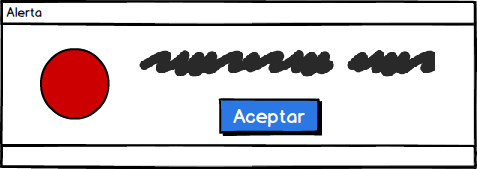
\includegraphics[width=0.5\textwidth]{./diseno/vescenarios/imagenes/alerta}
	\caption{Alerta Datos Erróneos - Vista de Escenarios}
	\label{fig:Alerta1 - Vista de Escenarios}
\end{figure}
\clearpage
\subsection{CU2 Visualizar Menú}
Al momento de ingresar las credenciales y que el sistema otorgue acceso al usuario, aparecerá una pantalla muy simular a la que mostramos a continuación (figura \ref{fig:Pantalla Visualizar Menu - Vista de Escenarios}). Esta pantalla posee el mismo diseño que el inicio de sesión (figura \ref{fig:Pantalla Iniciar Sesion - Vista de Escenarios}), solo que esta vez, se muestran tres opciones principales. 
\begin{itemize}
	\item \textbf{Gestionar Agenda:} En esta opción se desplegará otra pantalla que le dará acceso al usuario a toda la información que desee saber sobre los registros de los vehículos que estén dentro del taller además de la gestión de los mismos.
	\item \textbf{Gestionar Refacciones:} En dado caso que el usuario desee saber sobre la existencia de alguna refacción en particular dentro del almacén del taller además de generar una solicitud para la obtención de una si en necesario.
	\item \textbf{Cancelar:} El usuario desea salir de esa pantalla y regresar a la pantalla de Iniciar Sesión (figura \ref{fig:Pantalla Iniciar Sesion - Vista de Escenarios}).
\end{itemize}
\begin{figure}[!h]
	\centering
	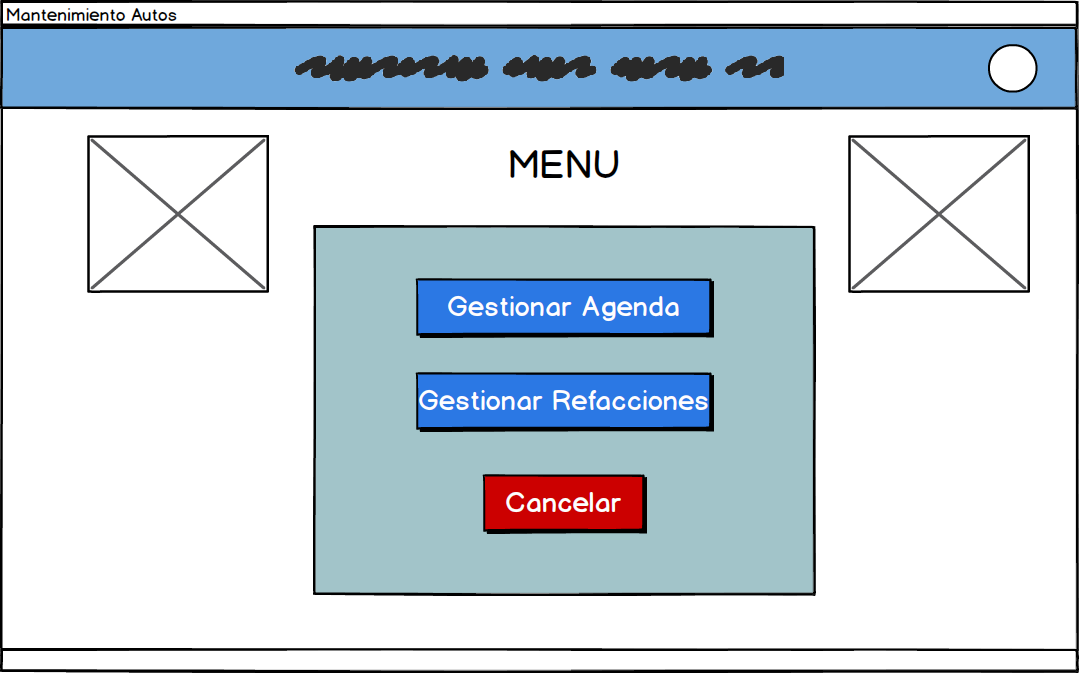
\includegraphics[width=1\textwidth]{./diseno/vescenarios/imagenes/VisualizarMenu}
	\caption{Pantalla Visualizar Menu - Vista de Escenarios}
	\label{fig:Pantalla Visualizar Menu - Vista de Escenarios}
\end{figure}
\clearpage
\subsection{CU3 Visualizar Agenda}
Supongamos que el usuario decide ver todos los registros de los vehículos dentro del taller y elige la opción de Gestionar Agenda, inmediatamente esta pantalla (figura \ref{fig:Pantalla Visualizar Agenda - Vista de Escenarios}) aparecerá. Compuesta principalmente por una tabla donde se mostrarán a manera de lista cada uno de los registros que estén almacenados en la base de datos, en caso de que no exista ningún registro, dicha tabla se mostrará vacía.
\\
En la parte superior derecha hay una barra de búsqueda, se explica a detalle este proceso mas adelante (véase \ref{sub:buscar registro}). 
\\
En la parte inferior se despliegan una serie de botones que permitirán al usuario gestionar esta tabla de registros que se le presentan:
\begin{itemize}
	\item \textbf{Actualizar Registro:} Permite al usuario actualizar la tabla una vez que este haya realizado algún cambio en los registros.
	\item \textbf{Registrar Vehículo:} Despliega una pantalla con un formulario de registro.
	\item \textbf{Modificar Vehículo:} Despliega una pantalla con un formulario de actualización.
	\item \textbf{Eliminar Vehículo:} Despliega una pantalla con un 'mensaje de seguridad'. 
	\item \textbf{Salir:} Regresar al menú de opciones (figura \ref{fig:Pantalla Visualizar Menu - Vista de Escenarios}). 
\end{itemize}
\begin{figure}[!h]
	\centering
	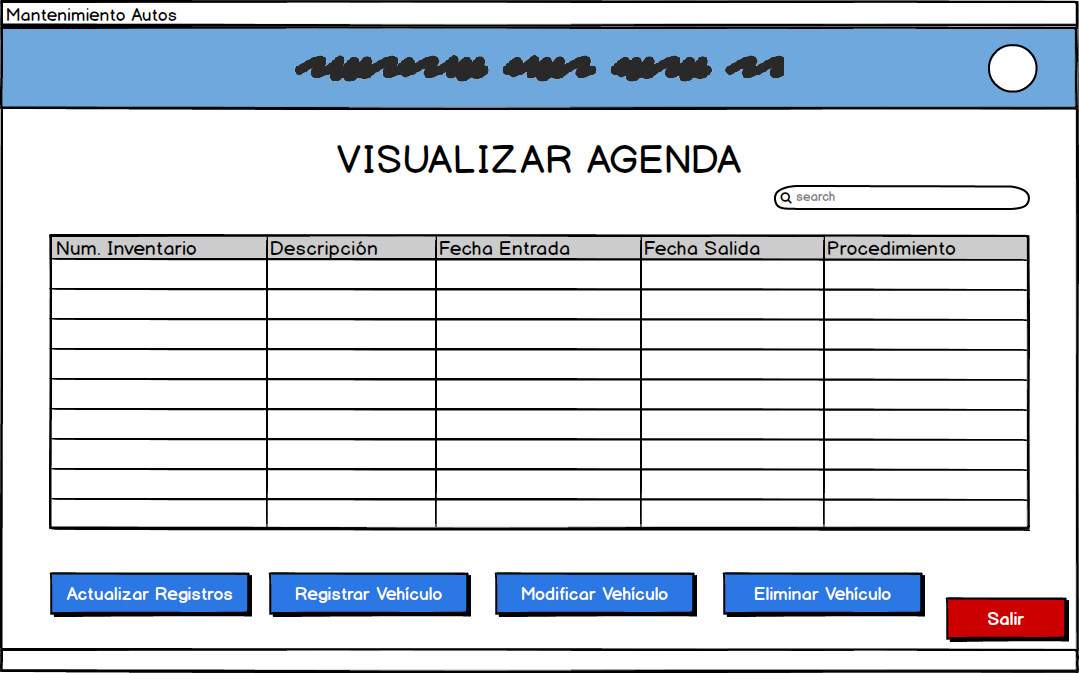
\includegraphics[width=1\textwidth]{./diseno/vescenarios/imagenes/VisualizarAgenda}
	\caption{Pantalla Visualizar Agenda - Vista de Escenarios}
	\label{fig:Pantalla Visualizar Agenda - Vista de Escenarios}
\end{figure}
Cabe señalar que el usuario debe de elegir un registro en la tabla para poder realizar alguna de las acciones antes mencionadas, de lo contrario aparecerá un 'mensaje de alerta' (figura \ref{fig:Alerta - Vista de Escenarios}) donde le de a entender al usuario lo que debe de hacer antes de relizar cualquier acción sobre algún registro.
\begin{figure}[!h]
	\centering
	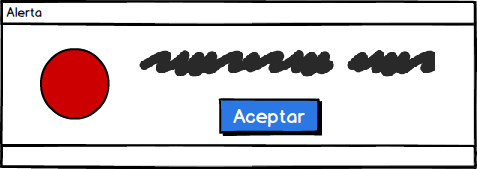
\includegraphics[width=0.5\textwidth]{./diseno/vescenarios/imagenes/alerta}
	\caption{Alerta Elección de Registro - Vista de Escenarios}
	\label{fig:Alerta - Vista de Escenarios}
\end{figure}
\clearpage
\subsection{CU4 Registrar Entrada de Vehículo}
Pantalla que aparece al presionar el botón de 'Registrar Vehículo' en la visualización de agenda (figura \ref{fig:Pantalla Visualizar Menu - Vista de Escenarios}). Este formulario le solicita al usuario los siguientes campos: Número de Inventario, Descripción, Fecha de Entrada, Fecha de Salida y el Procedimiento que se le hará al vehículo. 
\\
Cuenta con dos botones en la parte inferior, uno para proceder a enviar el registro a la base de datos y otro para cancelar en caso de que el usuario así lo desee. 
\\
\begin{figure}[!h]
	\centering
	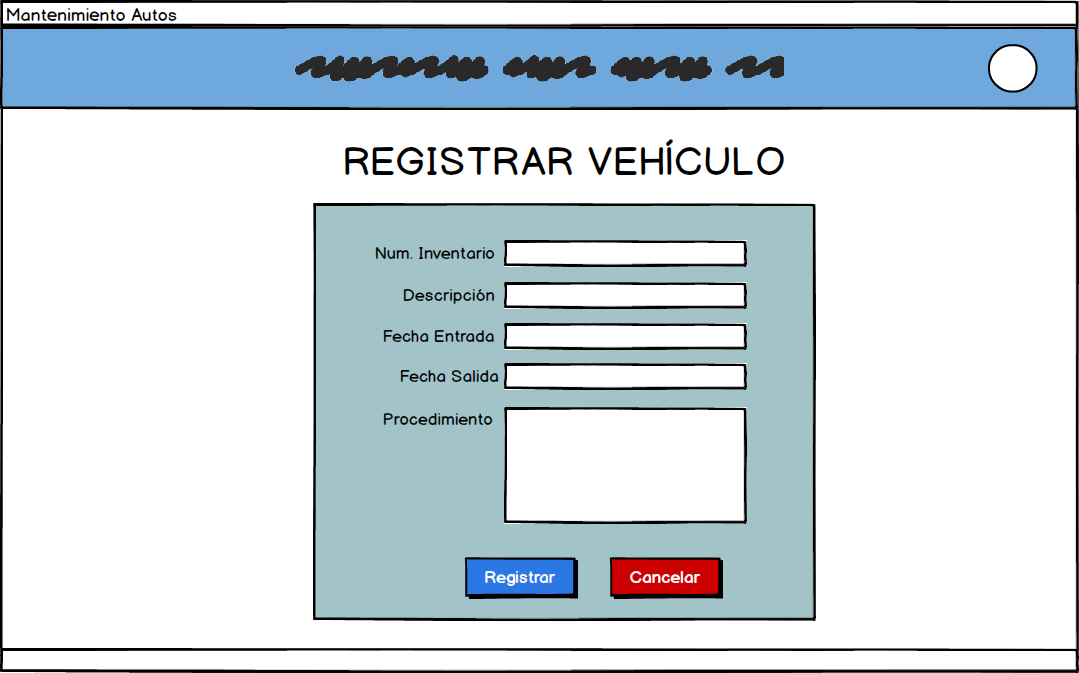
\includegraphics[width=0.9\textwidth]{./diseno/vescenarios/imagenes/registrarVehiculo}
	\caption{Pantalla Registrar Vehículo - Vista de Escenarios}
	\label{fig:Pantalla Registrar Vehículo - Vista de Escenarios}
\end{figure}
\\
En caso de que el usuario ingrese algún dato mal, es decir, que los campos no estén llenos o el formato de la información no es el correcto, aparecerá una alerta como la que se muestra a continuación (figura \ref{fig:Alerta2 - Vista de Escenarios}):
\begin{figure}[!h]
	\centering
	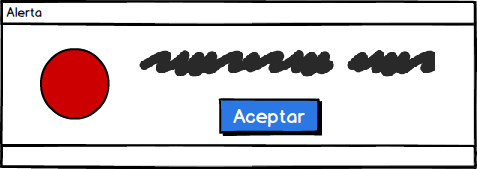
\includegraphics[width=0.4\textwidth]{./diseno/vescenarios/imagenes/alerta}
	\caption{Alerta Confirmación de Registro - Vista de Escenarios}
	\label{fig:Alerta2 - Vista de Escenarios}
\end{figure}
\clearpage
\subsection{CU5 Modificar Registro de Vehículo}
Esta pantalla es muy similar a la del 'Registro de Vehículo' (figura \ref{fig:Pantalla Registrar Vehículo - Vista de Escenarios}), solo que esta vez cuando el usuario desee modificar un registro en específico este formulario aparecerá con todos los campos llenos para que el usuario pueda modificar el que necesite. 
\\
En la parte inferior de la pantalla hay dos botones; el primero de ellos, el botón 'Modificar' lleva la información a la base de datos. El segundo, botón 'Cancelar' cierra esta pantalla y no hay alteración en los datos. 
\begin{figure}[!h]
	\centering
	\includegraphics[width=1\textwidth]{./diseno/vescenarios/imagenes/modificarVehículo}
	\caption{Pantalla Modificar Registro de Vehículo - Vista de Escenarios}
	\label{fig:Pantalla Modificar Registro de Vehículo - Vista de Escenarios}
\end{figure}
\\
En caso de que el usuario actualice algún dato mal, es decir, que los campos no estén llenos o el formato de la información no es el correcto, aparecerá una alerta como la que se muestra a continuación (figura \ref{fig:Alerta3 - Vista de Escenarios}):
\begin{figure}[!h]
	\centering
	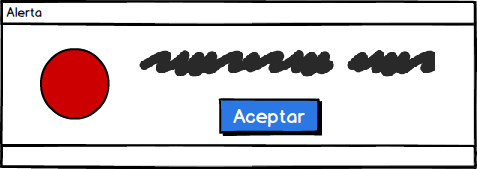
\includegraphics[width=0.5\textwidth]{./diseno/vescenarios/imagenes/alerta}
	\caption{Alerta Modificación - Vista de Escenarios}
	\label{fig:Alerta3 - Vista de Escenarios}
\end{figure}
\clearpage
\subsection{CU6 Eliminar Registro de Vehículo}
Esta pantalla es muy similar a la de Registrar Vehículo (figura \ref{fig:Pantalla Registrar Vehículo - Vista de Escenarios}) y a la de Modificar Vehículo (figura \ref{fig:Pantalla Modificar Registro de Vehículo - Vista de Escenarios}), sin embargo, esta pantalla esta diseñada para ser un 'mensaje de seguridad'. Muestra los datos que el usuario desea eliminar y al pulsar el botón 'Aceptar', el sistema ordena a la base de datos eliminar ese registro. Por otro lado, el botón 'Cancelar', cierra ese mensaje de seguridad y volvemos a la pantalla de Visualizar Agenda (figura \ref{fig:Pantalla Visualizar Agenda - Vista de Escenarios}).
\\
\begin{figure}[!h]
	\centering
	\includegraphics[width=1\textwidth]{./diseno/vescenarios/imagenes/eliminarVehículo}
	\caption{Pantalla Eliminar Registro de Vehículo - Vista de Escenarios}
	\label{fig:Pantalla Eliminar Registro de Vehículo - Vista de Escenarios}
\end{figure}
\\
Cuando se ha eliminado el registro de manera exitosa en la base de datos, el sistema mostrará una alerta (figura \ref{fig:Alerta4 - Vista de Escenarios}) como confirmación de que se ha borrado el registro de la base de datos.
\begin{figure}[!h]
	\centering
	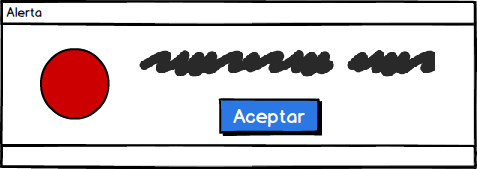
\includegraphics[width=0.5\textwidth]{./diseno/vescenarios/imagenes/alerta}
	\caption{Alerta Confirmación de Eliminación- Vista de Escenarios}
	\label{fig:Alerta4 - Vista de Escenarios}
\end{figure}
\subsection{CU7 Buscar Registro de Vehículo \label{sub:buscar registro}}
En este proceso no existe una pantalla como tal simplemente en la Visualización de la Agenda (figura \ref{fig:Pantalla Visualizar Agenda (busqueda)- Vista de Escenarios}) hay una barra de búsqueda en la parte superior donde el usuario podrá teclear el Número de Inventario del vehículo que desee. Si existe ese registro dentro de la base de datos, el sistema lo mostrará en la tabla. Caso contrario, si no existe, mostrará la tabla vacía. 
\begin{figure}[!h]
	\centering
	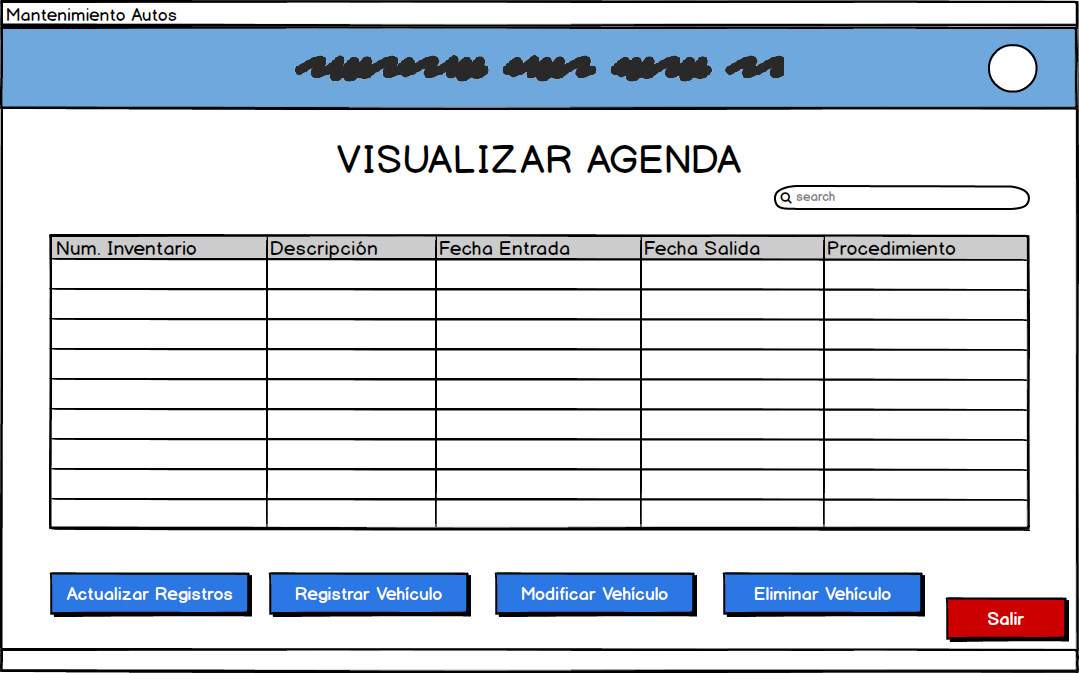
\includegraphics[width=1\textwidth]{./diseno/vescenarios/imagenes/VisualizarAgenda}
	\caption{Pantalla Visualizar Agenda (Búsqueda) - Vista de Escenarios}
	\label{fig:Pantalla Visualizar Agenda (busqueda)- Vista de Escenarios}
\end{figure}
\clearpage
\subsection{CU8 Visualizar Refacciones Disponibles}
Regresando un poco a la pantalla de Visualización del Menú (figura \ref{fig:Pantalla Visualizar Menu - Vista de Escenarios}), al pulsar el botón de 'Gestionar las Refacciones', aparece esta pantalla. Muy simular a la visualización de los registros pero aquí el usuario solamente podrá ver y buscar las refacciones que hay en existencia en el almacén del taller. En caso de que no exista alguno, podrá presionar el botón de la parte inferior 'Solicitar Refacción'.
\\
En la tabla el usuario podrá observar los registros a manera de lista dentro de una tabla, con los campos: Num. de Solicitud, una Descripción, la Fecha de Solicitud y la Existencia en almacén. 
\\
Al presionar el botón de salir, el sistema cerrará esta pantalla y regresará a la Visualización del Menú. 
\begin{figure}[!h]
	\centering
	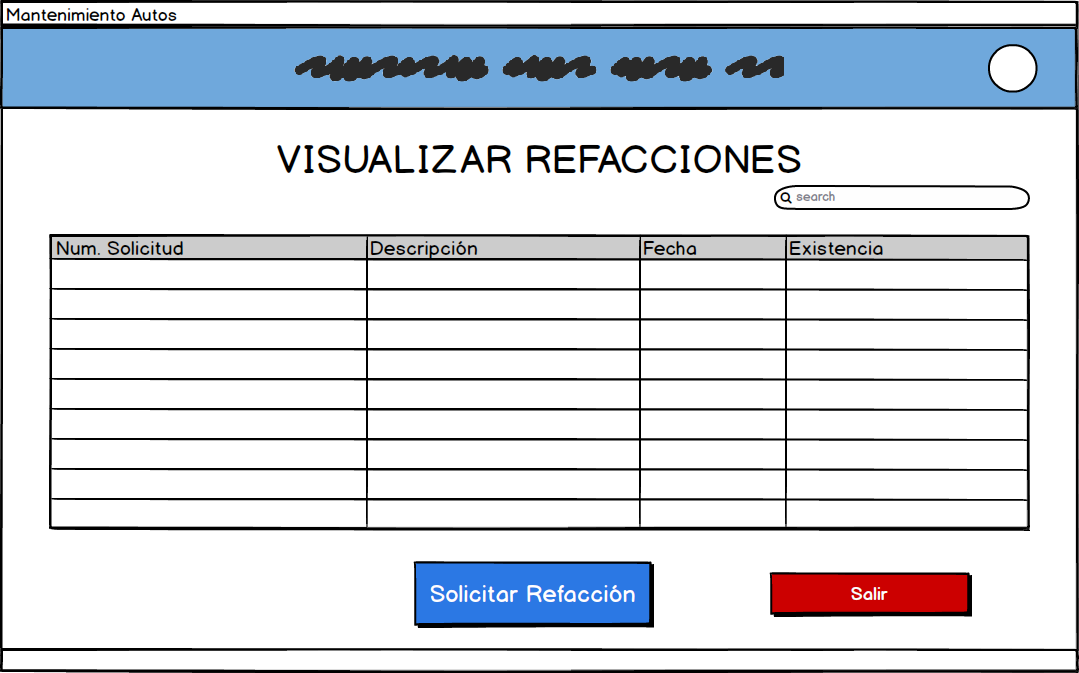
\includegraphics[width=1\textwidth]{./diseno/vescenarios/imagenes/VisualizarRefacciones}
	\caption{Pantalla Visualizar Refacciones - Vista de Escenarios}
	\label{fig:Pantalla Visualizar Refaccioes - Vista de Escenarios}
\end{figure}
\clearpage
\subsection{CU9 Solicitar Refacción}
Al entrar a esta parte del sistema, se despliega esta pantalla. Es un formulario de registro para la solicitud de alguna pieza en especifico. Solicitará un identificador (en este caso manejamos un Número de Solicitud), la Fecha en que se solicita y una Descripción donde se podrá agregar alguna otra información como el nombre o modelo. 
\\
Un vez llenado el formulario el usuario podrá pulsar el botón de 'Solicitar' para registrar esto en la base de datos. En caso de que el usuario desee salir de esta pantalla, simplemente deberá pulsar el botón 'Cancelar'.
\begin{figure}[!h]
	\centering
	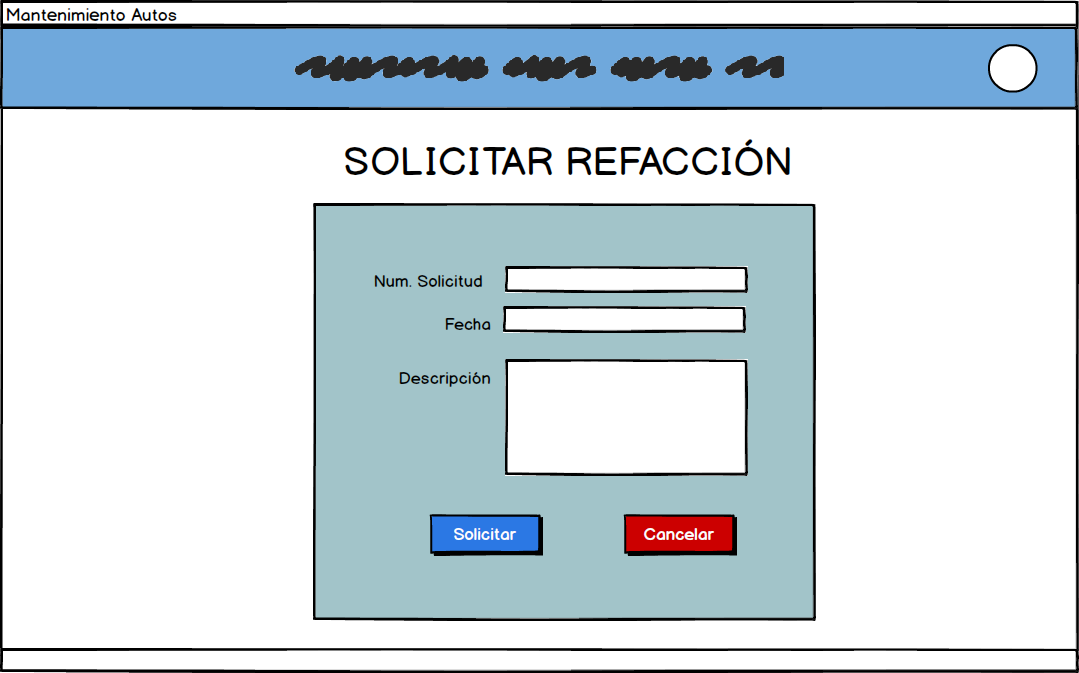
\includegraphics[width=1\textwidth]{./diseno/vescenarios/imagenes/solicitarRefaccion}
	\caption{Pantalla Solicitar Refacción - Vista de Escenarios}
	\label{fig:Pantalla Solicitar Refaccion - Vista de Escenarios}
\end{figure}
En caso de que el usuario ingrese de manera incorrecta alguno de los campos, el sistema mostrará un 'mensaje de alerta' (figura \ref{fig:Alerta5 - Vista de Escenarios}) informado del error que ha cometido. 
\begin{figure}[!h]
	\centering
	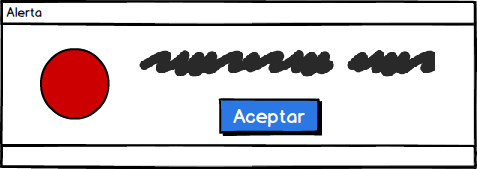
\includegraphics[width=0.4\textwidth]{./diseno/vescenarios/imagenes/alerta}
	\caption{Alerta Confirmación de Registro - Vista de Escenarios}
	\label{fig:Alerta5 - Vista de Escenarios}
\end{figure}
\subsection{CU10 Visualizar Empleados}
Cuando el administrador selecciona la opción 'Gestionar Empleados' del menú (figura \ref{fig:Pantalla Visualizar Menu Administrador - Vista de Escenarios}) aparece en pantalla la siguiente ventana. En ella se podrán visualizar a todos los empleados que están registrados dentro de la base de datos y que, obviamente, están trabajando dentro del taller. En la parte inferior de la ventana, existen más botones.
\begin{itemize}
	\item \textbf{Actualizar Registros:} Cuando se haga una acción en alguno de los registros, es necesario presionar este botón para que se actualicen todos los datos de la tabla-
	\item \textbf{Registrar Empleado:} Cuando se presiona este botón aparece una nueva ventana donde se podrá ingresar los datos de un nuevo empleado.
	\item \textbf{Modificar Empleado:} Al seleccionar una fila de la tabla (a un empleado registrado), aparecerá una ventana con un formulario de actualización.
	\item \textbf{Eliminar Empleado:} Al seleccionar una fila de la tabla (empleado registrado), aparecerá una ventana con un mensaje de seguridad para verificar si realmente se desea eliminar ese registro.
	\item \textbf{Salir:} El administrador cierra esa ventana y al mismo tiempo regresa al menú, figura \ref{fig:Pantalla Visualizar Menu Administrador - Vista de Escenarios}.
\end{itemize}
\begin{figure}[!h]
	\centering
	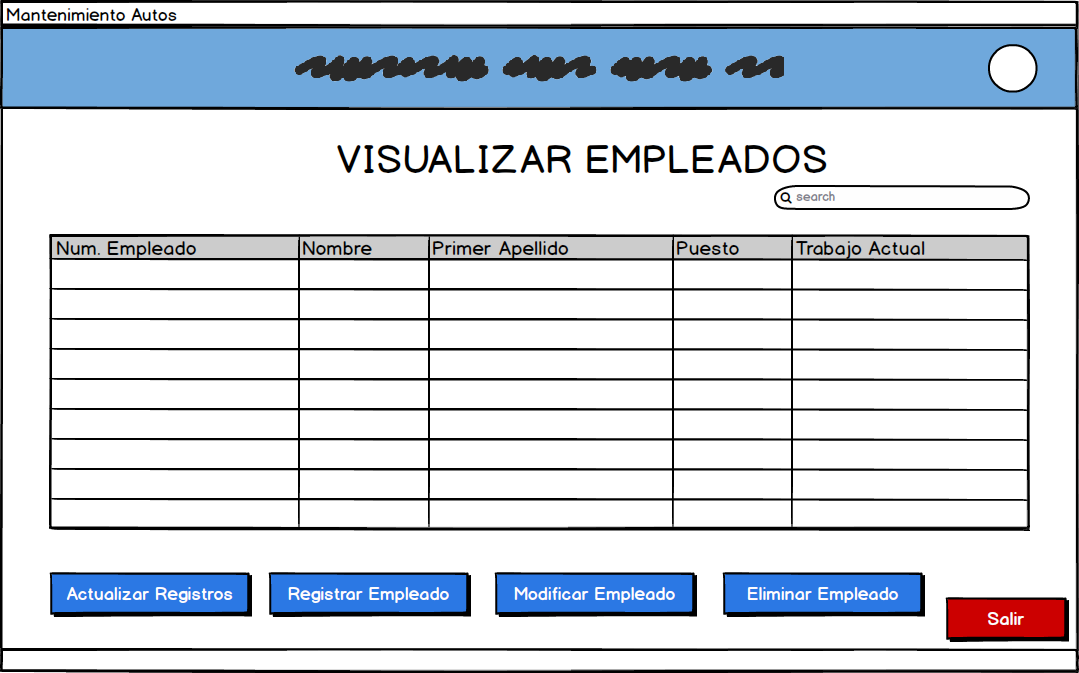
\includegraphics[width=1\textwidth]{./diseno/vescenarios/imagenes/VisualizarEmpleados}
	\caption{Pantalla Visualizar Empleados - Vista de Escenarios}
	\label{fig:Pantalla Visualizar Empleados - Vista de Escenarios}
\end{figure}
En dado caso de que se quiera modificar o eliminar un registro y no se ha seleccionado un renglón de la tabla, aparecerá un mensaje de alerta que le dirá al administrador que debe de seleccionar un registro.
\begin{figure}[!h]
	\centering
	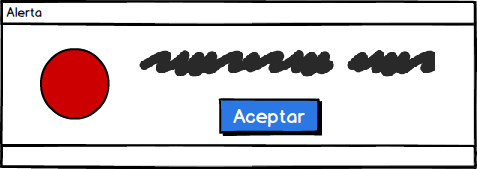
\includegraphics[width=0.5\textwidth]{./diseno/vescenarios/imagenes/alerta}
	\caption{Alerta - Vista de Escenarios}
	\label{fig:Alerta Empleados - Vista de Escenarios}
\end{figure}
\clearpage
\subsection{CU 11 Registrar Empleado}
En la siguiente ventana, figura \ref{fig:Pantalla Registrar Empleado - Vista de Escenarios}, se muestra un formulario de registro para un nuevo empleado donde el administrador podrá ingresar la información que el sistema le solicita para llevar a cabo el registro. Los datos que pide son: número de empleado (este será el usuario de cuenta del empleado), nombre completo y una contraseña que se le proporcionará al empleado una vez que el registro se haya hecho. En la parte inferior de la ventana, tenemos dos botones:
\begin{itemize}
	\item \textbf{Registrar:} Una vez llenados los campos, al dar click en este botón el sistema los validará y verificará si todos están llenos y con el formato adecuado, de no ser así se mostrará un mensaje de error (figura \ref{fig:Alerta Registro Empleados - Vista de Escenarios}) y el administrador debe de corregir el error de captura.
	\item \textbf{Cancelar: } El administrador desea salir de esa ventana, y el sistema regresa al a ventana 'Visualizar Empleados' (figura \ref{fig:Pantalla Visualizar Empleados - Vista de Escenarios}).
\end{itemize}
\begin{figure}[!h]
	\centering
	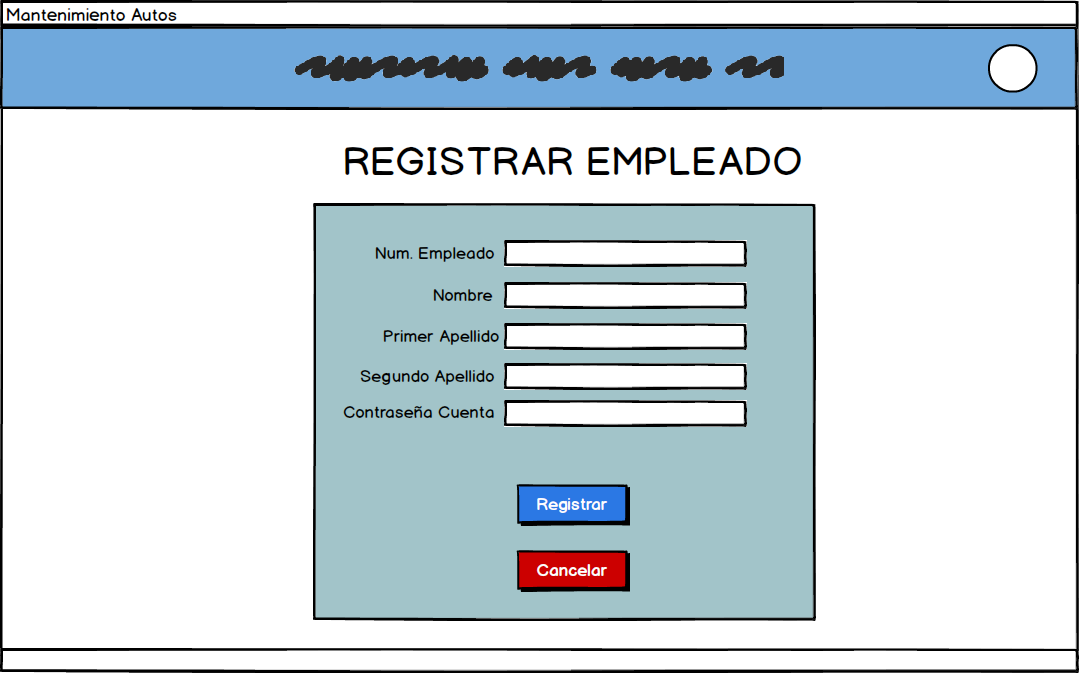
\includegraphics[width=0.8\textwidth]{./diseno/vescenarios/imagenes/registrarEmpleado}
	\caption{Pantalla Registrar Empleado - Vista de Escenarios}
	\label{fig:Pantalla Registrar Empleado - Vista de Escenarios}
\end{figure}
\begin{figure}[!h]
	\centering
	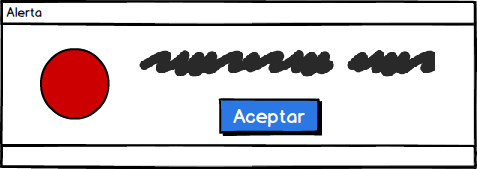
\includegraphics[width=0.3\textwidth]{./diseno/vescenarios/imagenes/alerta}
	\caption{Alerta Registro Empleados - Vista de Escenarios}
	\label{fig:Alerta Registro Empleados - Vista de Escenarios}
\end{figure}
\clearpage
\subsection{CU12 Modificar Empleado}
Al momento de seleccionar un registro de la pantalla de 'Visualizar Empleados' (figura \ref{fig:Pantalla Visualizar Empleados - Vista de Escenarios}) y seleccionar la opción de modificar el registro del empleado, se mostrará la ventana de modificación, la cual contiene un formulario de actualización de los datos. Cada uno de los campos estará lleno con la información que esta guardada dentro de la base de datos. El administrador podrá modificar dicha información y podrá seleccionar alguno de los botones de la parte inferior de la pantalla:
\begin{itemize}
	\item \textbf{Modificar:} Al dar click en esta opción, el sistema valida si toda la información es correcta (formato, estructura y si los campos están llenos). En caso de que no sea así, el sistema mostrará una alerta (figura \ref{fig:Alerta Modificar Empleado - Vista de Escenarios}).
	\item \textbf{Cancelar:} Salir de esa ventana y regresar a al pantalla anterior. (Figura \ref{fig:Pantalla Visualizar Empleados - Vista de Escenarios}).
\end{itemize}
\begin{figure}[!h]
	\centering
	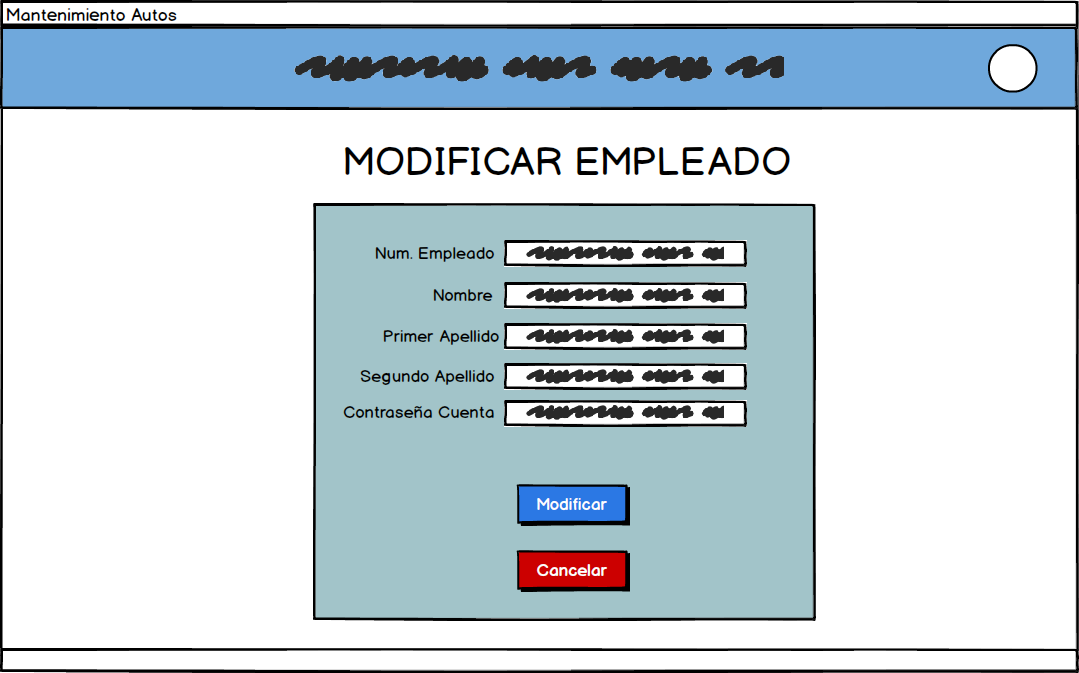
\includegraphics[width=0.8\textwidth]{./diseno/vescenarios/imagenes/modificarEmpleado}
	\caption{Pantalla Modificar Empleado - Vista de Escenarios}
	\label{fig:Pantalla Modificar Empleado - Vista de Escenarios}
\end{figure}
\begin{figure}[!h]
	\centering
	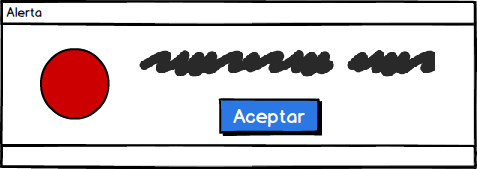
\includegraphics[width=0.3\textwidth]{./diseno/vescenarios/imagenes/alerta}
	\caption{Alerta Modificar Empleado - Vista de Escenarios}
	\label{fig:Alerta Modificar Empleado - Vista de Escenarios}
\end{figure}
\clearpage
\subsection{CU13 Eliminar Empleado}
Esta pantalla funciona como un mensaje de seguridad. Al seleccionar un registro de la pantalla 'Visualizar Empleado' y el administrador selecciona la opción de eliminar empleado, se mostrará la siguiente pantalla. Aqui se muestran los datos del empleado que se desea eliminar y dos opciones:
\begin{itemize}
	\item \textbf{Aceptar:} El sistema interactúa con la base de datos y se logra eliminar el registro del empleado. Una vez eliminado, el sistema mostrará un mensaje que el proceso a sido exitoso. (Figura \ref{fig:Alerta Eliminar Empleado - Vista de Escenarios}).
	\item \textbf{Cancelar:} 
\end{itemize}
\begin{figure}[!h]
	\centering
	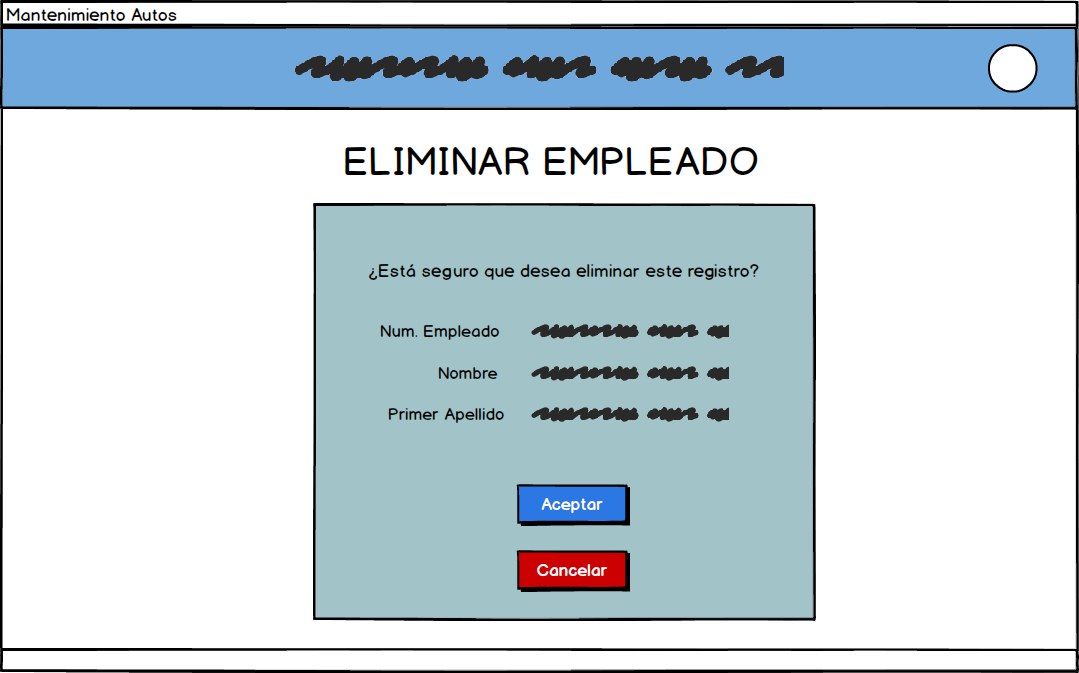
\includegraphics[width=0.8\textwidth]{./diseno/vescenarios/imagenes/eliminarEmpleado}
	\caption{Pantalla Eliminar Empleado - Vista de Escenarios}
	\label{fig:Pantalla Eliminar Empleado - Vista de Escenarios}
\end{figure}
\begin{figure}[!h]
	\centering
	\includegraphics[width=0.5\textwidth]{./diseno/vescenarios/imagenes/alerta}
	\caption{Alerta Eliminar Empleado - Vista de Escenarios}
	\label{fig:Alerta Eliminar Empleado - Vista de Escenarios}
\end{figure}
\clearpage
\subsection{CU14 Buscar Empleado}
Para este proceso, el sistema no tiene destinado una pantalla completamente, solo es una pequeña barra de búsqueda en la parte superior derecha de la pantalla 'Visualizar Empleados' (figura \ref{fig:Pantalla Visualizar Empleado (Busqueda) - Vista de Escenarios}). En dicha barra, el administrador podrá ingresar el Número de Empleado que desee. Si existe el registro dentro de la base de datos, el sistema lo mostrara directamente en la tabla. Caso contrario, mostrará la tabla vacía.
\begin{figure}[!h]
	\centering
	\includegraphics[width=1\textwidth]{./diseno/vescenarios/imagenes/visualizarEmpleados}
	\caption{Pantalla Visualizar Empleado (Búsqueda) - Vista de Escenarios}
	\label{fig:Pantalla Visualizar Empleado (Busqueda) - Vista de Escenarios}
\end{figure}
\clearpage
\subsection{CU15 Visualizar Refacciones}
En esta ventana, el administrador puede visualizar todas las refacciones que se encuentran dentro del almacén del taller. Esta tabla posee tres columnas, el Número de Inventario de la refacción, la descripción de la misma refacción y por último el vehículo para el que se necesita. En la parte inferior de la ventana tenemos varias opciones:
\begin{itemize}
	\item \textbf{Actualizar Registros:} Una vez que se haya realizado una acción con algún registro de la tabla, el administrador debe de dar click en este botón para que todas las filas y columnas de la tabla se actualicen.
	\item \textbf{Registrar Refacción:} Se despliega una pantalla donde el administrador podrá ingresar los datos necesarios para hacer un registro de una refacción.
	\item \textbf{Modificar Refacción:} En caso de que se necesite modificar por alguna razón un registro de refacción se podrá hacer con esta ocpción.
	\item \textbf{Eliminar Refacción:} Cuando se requiera eliminar un registro de una refacción por la razón que sea, esta opción ayudará al administrador a hacerlo desplegando un mensaje de seguridad.
	\item \textbf{Salir: }El sistema regresará a la ventana del menú del administrador, figura \ref{fig:Pantalla Visualizar Menu Administrador - Vista de Escenarios}. 
\end{itemize}
En caso de que no se seleccione una fila dentro de la tabla y se desee modificar o eliminar algún registro de la refacción se mostrará un mensaje de error y el administrador será enterado del error que está cometiendo. 
\begin{figure}[!h]
	\centering
	\includegraphics[width=1\textwidth]{./diseno/vescenarios/imagenes/VisualizasRefacciones}
	\caption{Pantalla Visualizar Refacciones Administrador - Vista de Escenarios}
	\label{fig:Pantalla Visualizar Refacciones Administrador - Vista de Escenarios}
\end{figure}
\begin{figure}[!h]
	\centering
	\includegraphics[width=0.5\textwidth]{./diseno/vescenarios/imagenes/alerta}
	\caption{Alerta Refacciones- Vista de Escenarios}
	\label{fig:Alerta Refacciones - Vista de Escenarios}
\end{figure}
\clearpage
\subsection{CU16 Registrar Refacción}
Esta pantalla aparece cuando el administrador elige la opción de registrar una refacción desde la pantalla de 'Visualizar Refacciones, (figura\ref{fig:Pantalla Visualizar Refacciones Administrador - Vista de Escenarios}). En esta sección, el sistema solicita que el administrador ingrese la información para hacer el registro eb este caso es el Número de Inventario, para que Vehículo va destinado y por último una descripción de la refacción que se va a utilizar. En la parte inferior de la pantalla, tenemos dos botones con diferentes opciones:
\begin{itemize}
	\item \textbf{Registrar:} Al dar click en este botón, el sistema validará cada uno de los campos que han sido llenados, su formato y su contenido. En caso de que exista un error, el propio sistema mostrará un mensaje de error para que el administador corrija el error.
	\item \textbf{Cancelar:} El sistema regresa a la pantalla anterior \ref{fig:Pantalla Visualizar Refacciones Administrador - Vista de Escenarios} sin hacer algún registro.
\end{itemize} 
\begin{figure}[!h]
	\centering
	\includegraphics[width=0.8\textwidth]{./diseno/vescenarios/imagenes/registrarRefacciones}
	\caption{Pantalla Registrar Refacción - Vista de Escenarios}
	\label{fig:Pantalla Registrar Refacción - Vista de Escenarios}
\end{figure}
\begin{figure}[!h]
	\centering
	\includegraphics[width=0.3\textwidth]{./diseno/vescenarios/imagenes/alerta}
	\caption{Alerta Registro Refacciones- Vista de Escenarios}
	\label{fig:Alerta Registro Refacciones - Vista de Escenarios}
\end{figure}
\subsection{CU17 Modificar Refacción}
Cuando el administrador elige la opción de modificar un registro, se despliega esta pantalla donde el sistema muestra un formulario de actualización donde todos los campos están llenos con la información que está dentro de la base de datos. En la parte inferior de esta ventana tenemos dos botones:
\begin{itemize}
	\item \textbf{Modificar:} Al dar click en este botón, el sistema validará nuevamente todos los campos hayan sido modificados o no, validando si están llenos y su formato. 
	\item \textbf{Cancelar:} El sistema regresa a la pantalla anterior (figura \ref{fig:Pantalla Visualizar Refacciones Administrador - Vista de Escenarios}) sin modificar ningún dato. 
\end{itemize}
\begin{figure}[!h]
	\centering
	\includegraphics[width=0.8\textwidth]{./diseno/vescenarios/imagenes/modificarRefaccion}
	\caption{Pantalla Modificar Refacciones  - Vista de Escenarios}
	\label{fig:Pantalla Modificar Refacción - Vista de Escenarios}
\end{figure}
\begin{figure}[!h]
	\centering
	\includegraphics[width=0.3\textwidth]{./diseno/vescenarios/imagenes/alerta}
	\caption{Alerta Modificar Refacciones- Vista de Escenarios}
	\label{fig:Alerta Registro Refacciones - Vista de Escenarios}
\end{figure}
\clearpage
\subsection{CU18 Eliminar Refacción}
Esta pantalla funciona como un mensaje de seguridad, este se asegurará que el administrador realmente quiere eliminar el registro que ha seleccionado de una refacción, mostrará toda la información que se tiene sobre esa refacción. En la parte inferior hay dos botones:
\begin{itemize}
	\item \textbf{Aceptar:} El sistema elimina el registro seleccionado por el administrador y muestra un mensaje de confirmación que el proceso ha sido exitoso.
	\item \textbf{Cancelar:} El sistema regresa a la pantalla anterior (figura \ref{fig:Pantalla Visualizar Refacciones Administrador - Vista de Escenarios}) sin hacer alguna modificación.
\end{itemize}
{\begin{figure}[!h]
	\centering
	\includegraphics[width=0.8\textwidth]{./diseno/vescenarios/imagenes/eliminarRefaccion}
	\caption{Pantalla Eliminar Refacciones  - Vista de Escenarios}
	\label{fig:Pantalla Eliminar Refacción - Vista de Escenarios}
\end{figure}
\begin{figure}[!h]
	\centering
	\includegraphics[width=0.3\textwidth]{./diseno/vescenarios/imagenes/alerta}
	\caption{Alerta Eliminar Refacciones- Vista de Escenarios}
	\label{fig:Alerta Eliminar Refacciones - Vista de Escenarios}
\end{figure}
\clearpage
\subsection{CU19 Buscar Refacciones}
Para la búsqueda de una refacción el sistema no tiene un módulo destinado como tal, es simplemente una barra de búsqueda en la parte superior derecha donde el administrador podrá ingresar el número de inventario de alguna refacción, en caso de que exista se mostrará la información en la tabla si no es así, la tabla se mostrará vacía. 
\begin{figure}[!h]
	\centering
	\includegraphics[width=0.8\textwidth]{./diseno/vescenarios/imagenes/visualizarRefacciones}
	\caption{Pantalla Visualizar Refacciones Admin (Búsqueda) - Vista de Escenarios}
	\label{fig:Pantalla refacciones busqueda- Vista de Escenarios}
\end{figure}
\clearpage
\subsection{CU20 Visualizar Solicitudes}
En esta pantalla, el administrador podrá visualizar en una tabla cada una de las solicitudes de refacción que los empleados han hecho. Esta tabla consta de tres columnas, la primera es el número de Inventario de la refacción, la segunda es el nombre del empleado que solicitó la refacción y la tercera es una descripción de la refacción. Solo consta de tres opciones en la parte inferior de la ventana:
\begin{itemize}
	
	\item \textbf{Atender Solicitud:} En esta opción se desplegará una pantalla donde el administrador podrá verificar la solicitud y aceptarla. En caso de que no se elija una fila de la tabla, se mostrará un mensaje de error en pantalla. (Figura \ref{fig:Alerta Solicitudes - Vista de Escenarios}).
	\item \textbf{Salir:} Regresará a la pantalla anterior la cual es el Menú del administrador (figura \ref{fig:Pantalla Visualizar Menu Administrador - Vista de Escenarios}).
\end{itemize}
\begin{figure}[!h]
	\centering
	\includegraphics[width=0.8\textwidth]{./diseno/vescenarios/imagenes/visualizarSolicitudes}
	\caption{Pantalla Visualizar Solicitudes - Vista de Escenarios}
	\label{fig:Pantalla Visualizar Solicitudes- Vista de Escenarios}
\end{figure}
\begin{figure}[!h]
	\centering
	\includegraphics[width=0.3\textwidth]{./diseno/vescenarios/imagenes/alerta}
	\caption{Alerta Solicitudes- Vista de Escenarios}
	\label{fig:Alerta Solicitudes - Vista de Escenarios}
\end{figure}
\clearpage
\subsection{CU21 Atender Solicitud}
Esta pantalla mostrará todos los datos de la solicitud que se haya seleccionado, aquí el administrador podrá aprobar la solicitud una vez que el proveedor haya conseguido la refacción que se necesita. El botón de cancelar regresa a la pantalla anterior de visualizar solicitudes (figura \ref{fig:Pantalla Visualizar Solicitudes- Vista de Escenarios}) y el administrador podrá seguir interactuando con el sistema. 
\begin{figure}[!h]
	\centering
	\includegraphics[width=0.8\textwidth]{./diseno/vescenarios/imagenes/eliminarSolicitud}
	\caption{Pantalla Atender Solicitud - Vista de Escenarios}
	\label{fig:Pantalla Atender - Vista de Escenarios}
\end{figure}
\clearpage 
	\begin{thebibliography}{9}
	\bibitem{1}UML-ORG UML2-Diagramas UML Recuperado \today \hspace{0.1cm} de
	http://uml2.org 
	\bibitem{2}Philippe Kruchten Architectural Blueprints—The “4+1” View Model of Software Architecture Paper published in IEEE Software 12 (6) November 1995, pp. 42-50
\end{thebibliography}
	
	\appendix
	\appendixpage
	\chapter{Anexos del Documento}
\subsection{Product Backlog}
Para este documento, utilizamos una hoja de cálculo Excel para más comodidad y portabilidad. Primeramente se establecen las prioridades que se van a manejar dentro de los sprints para posteriormente categorizar cada historia de usuario o actividad con una de estas prioridades.
\begin{figure}[!h]
	\centering
	\includegraphics[width=1\textwidth]{./productBacklog/imagenes/prioridades}
	\caption{Prioridades del Product Backlog}
	\label{fig:Prioridades del Product Backlog}
\end{figure}
\subsubsection{Primer Sprint}
\begin{figure}[!h]
	\centering
	\includegraphics[width=1\textwidth]{./productBacklog/imagenes/primerSprint}
	\caption{Primer Sprint - Product Backlog}
	\label{fig:Primer Sprint - Product Backlog}
\end{figure}
\subsubsection{Segundo Sprint}
\begin{figure}[!h]
	\centering
	\includegraphics[width=1\textwidth]{./productBacklog/imagenes/segundoSprint}
	\caption{Segundo Sprint - Product Backlog}
	\label{fig:egundo Sprint - Product Backlog}
\end{figure}
\subsection{Sprint Backlog}
En este documento se planifica todo el ciclo de vida de desarrollo de cada módulo del sistema, integrando un ID, el nombre del módulo, la fecha de incio y fin del proceso y un responsable de ese proceso.
\subsubsection{Primer Sprint}
\begin{figure}[!h]
	\centering
	\includegraphics[width=1\textwidth]{./sprintBacklog/imagenes/sprint1}
	\caption{Primer Sprint - Sprint Backlog}
	\label{fig:Primer Sprint - Sprint Backlog}
\end{figure}
\clearpage
\subsubsection{Segundo Sprint}
\begin{figure}[!h]
	\centering
	\includegraphics[width=1\textwidth]{./sprintBacklog/imagenes/sprint2}
	\caption{Segundo Sprint - Sprint Backlog}
	\label{fig:egundo Sprint - Sprint Backlog}
\end{figure}
\subsection{Vistas del MVP}
A continuación se anexan las pantallas del sistema MVP que se ha implementado hasta ahora, los módulos que hasta ahora se han programado son:
\begin{itemize}
	\item Inicio de Sesión.
	\item Menú.
	\item Gestión de Vehículos.
	\item Visualización de Agenda (vehículos registrados).
	\item Registro de Vehículo.
	\item Modificar Vehículo.
	\item Eliminar Vehículo.
	\item Buscar un Vehículo (barra de búsqueda).
\end{itemize}
Si desea ver el código fuente y la documentación de todo el proyecto, ingrese a este enlace desde su navegar web preferido: \url{https://github.com/Ulysses2213/mantenimientoVehiculos} \\

Para descargar el MVP de los primeros 2 sprints del proyecto, ingrese a este enlace: \url{https://1drv.ms/u/s!AlSsvA47vIkMguhf_GCXbHVBdvvN_Q?e=Sj2tO2} \\

Para poder ejecutar el MVP es necesario descargar Java en su ultima versión, lo puede hacer desde este enlace: \url{https://www.java.com/es/}
\vspace{3cm}
\begin{figure}[!h]
	\centering
	\includegraphics[width=1\textwidth]{./apendice/imagenes/login}
	\caption{Captura de Pantalla MVP- Iniciar Sesión}
	\label{fig:Captura de Pantalla MVP- Iniciar Sesion}
\end{figure}
\clearpage
\begin{figure}
	\centering
	\includegraphics[width=1\textwidth]{./apendice/imagenes/menu}
	\caption{Captura de Pantalla MVP- Menú}
	\label{fig:Captura de Pantalla MVP- Menu}
\end{figure}

\begin{figure}
	\centering
	\includegraphics[width=1\textwidth]{./apendice/imagenes/agenda}
	\caption{Captura de Pantalla MVP- Visualizar Agenda}
	\label{fig:Captura de Pantalla MVP- Visualizar Agenda}
\end{figure}

\begin{figure}
	\centering
	\includegraphics[width=1\textwidth]{./apendice/imagenes/registro}
	\caption{Captura de Pantalla MVP- Registro de Vehículo}
	\label{fig:Captura de Pantalla MVP- Registro de Vehiculo}
\end{figure}

\begin{figure}
	\centering
	\includegraphics[width=1\textwidth]{./apendice/imagenes/modificar}
	\caption{Captura de Pantalla MVP- Modificar Vehículo}
	\label{fig:Captura de Pantalla MVP- Modificar Vehiculo}
\end{figure}

\begin{figure}
	\centering
	\includegraphics[width=1\textwidth]{./apendice/imagenes/eliminar}
	\caption{Captura de Pantalla MVP- Eliminar Vehículo}
	\label{fig:Captura de Pantalla MVP- Eliminar Vehiculo}
\end{figure}


\end{document}